\documentclass[11pt,a4paper,twoside,openright]{memoir}

%%%%%%%%%%%%%%%%%%%%%%%%%%%%%%%%%%%%%%%%%%%%%%%%%%%%%%%
%  In my opinion (DW) there are no fonts available in the standard
%  TeX/LaTeX set that are ideal for this use, unless you go down to 9pt or 
%  8pt for your text face, and this is too small.  If you have Metafont you
%  should consider generating a cmr17 font at a magstep of two (about 25pt)
%  or three (about 30pt), or even more, depending on the point size of your
%  main text.  Why not go the whole hog and design some really fancy 
%  capitals from scratch!
%
%%%%%%%%%%%%%%%%%%%%% BOX ONE %%%%%%%%%%%%%%%%%%%%%%%%%
%\typein[\dropinitialfont]{Font for Dropped initial:} %
%\font\largefont \dropinitialfont                     %
%%%%%%%%%%%%%%%%%%%%%%%%%%%%%%%%%%%%%%%%%%%%%%%%%%%%%%%
%
%%%%%%%%%%%%%%%%%%%%% BOX TWO %%%%%%%%%%%%%%%%%%%%%%%%%
%\font\largefont= cmr10 scaled \magstep5              %
%\font\largefont= cmbx10 scaled \magstep5             %
%\font\largefont= cmbx17 scaled \magstep3             %
\font\largefont= cmr17 scaled \magstep5               %
%%%%%%%%%%%%%%%%%%%%%%%%%%%%%%%%%%%%%%%%%%%%%%%%%%%%%%%

% Copyright Symbole u..
\def\TReg{\textsuperscript{\textregistered}}
\def\TCop{\textsuperscript{\textcopyright}}
\def\TTra{\textsuperscript{\texttrademark}}

\def\drop#1#2{{\noindent
    \setbox0\hbox{\largefont #1}\setbox1\hbox{#2}\setbox2\hbox{(}%
    \count0=\ht0\advance\count0 by\dp0\count1\baselineskip
    \advance\count0 by-\ht1\advance\count0by\ht2
    \dimen1=.5ex\advance\count0by\dimen1\divide\count0 by\count1
    \advance\count0 by1\dimen0\wd0
    \advance\dimen0 by.25em\dimen1=\ht0\advance\dimen1 by-\ht1
    \global\hangindent\dimen0\global\hangafter-\count0
    \hskip-\dimen0\setbox0\hbox to\dimen0{\raise-\dimen1\box0\hss}%
    \dp0=0in\ht0=0in\box0}#2}

% end of new \drop command
%%%%%%%%%%%%%%%%%%%%%%%%%%%%%%%%%%%%%%%%%%%%%%%%%%%%%%%

%%%%%%%%%%%%%%%%%%%%%%%%%%%%%%%%%%%%%%%%%%%%%%%%%%%%%%%
% new \versal command
\newcommand{\versal}[1]{{\noindent
    \setbox0\hbox{\largefont #1}%
    \count0=\ht0                   % height of versal
    \count1=\baselineskip          % baselineskip
    \divide\count0 by \count1      % versal height/baselineskip
    \dimen1 = \count0\baselineskip % distance to drop versal
    \advance\count0 by 1\relax     % no of indented lines
    \dimen0=\wd0                   % width of versal
    \global\hangindent\dimen0      % set indentation distance
    \global\hangafter-\count0      % set no of indented lines
    \hskip-\dimen0\setbox0\hbox to\dimen0{\raise-\dimen1\box0\hss}%
    \dp0=0in\ht0=0in\box0}}
% end of new \versal command
%%%%%%%%%%%%%%%%%%%%%%%%%%%%%%%%%%%%%%%%%%%%%%%


%%%%%%%%%%%%%%%%%%%%%%%%%%%%%%%%%%%%%%%%%%%%%%%
% redefining the textblocksize
%%%%%%%%%%%%%%%%%%%%%%%%%%%%%%%%%%%%%%%%%%%%%%%
\setlrmarginsandblock{1in}{1.5in}{*}
\checkandfixthelayout
%%%%%%%%%%%%%%%%%%%%%%%%%%%%%%%%%%%%%%%%%%%%%%%


\usepackage{graphicx}
\usepackage{latexsym}
\usepackage{epsfig}
\usepackage[figuresright]{rotating}
\usepackage{dsfont}
\usepackage{german}
\usepackage[utf8]{inputenc}
%\usepackage[dvips]{color}
\usepackage{colortbl}
	\definecolor{darkblue}{rgb}{0,0,0.4}
	\definecolor{darkgray}{rgb}{0.1,0.1,0.2}
	\definecolor{darkred}{rgb}{0.6,0.0,0.0}
   \definecolor{darkgreen}{rgb}{0.0,0.6,0.0}
   \definecolor{orange}{rgb}{1.0,0.8,0.0}

%---- for algorithms ----
\usepackage[Algorithmus]{algorithm}
\usepackage{algorithmic}

%---- for the index ----
\usepackage{layouts}[2001/04/29]
\makeindex

\usepackage{caption, booktabs}

\usepackage{hyperref}
\usepackage{memhfixc}
\hypersetup{colorlinks=true,linkcolor=darkgray,urlcolor=darkblue,citecolor=darkblue,filecolor=darkgreen}

%---- a second bibliography ----
\usepackage{multibib}
\renewcommand{\refname}{Allgemeine Literaturquellen}

%---- some new math symbols ----
\usepackage{nicefrac} % schräge bruchstriche
\usepackage{amssymb}
\newcommand{\Real}{\mathbb R}

%---- memoir package specialties
%\pagestyle{companion}
\pagestyle{Ruled}
\setlength{\epigraphwidth}{7cm}
\setcounter{tocdepth}{3}
\setcounter{secnumdepth}{3}
\maxsecnumdepth{subsection}

% change standard font
%\usepackage{cmbright}
\renewcommand{\rmdefault}{cmss}
\renewcommand{\sfdefault}{cmss}

% set figure resp. table name and number bold
\makeatletter
\renewcommand{\fnum@figure}{\textbf{\figurename~\thefigure}}
\renewcommand{\fnum@table}{\textbf{\tablename~\thetable}}
\makeatother

% setting the authors for a verse
\newcommand{\attrib}[1]{%
	\nopagebreak{\raggedleft\footnotesize #1\par}}

%---- general information ----
\author{ 
	\small{vorgelegt von} \vspace{.5cm} 											\\ 
	\Large{\textbf{Lukas Michael Müller}} 											\\ 
	\small{geb.\ in Schotten}}
\title{
	\textbf{\vspace{-2.5cm}
		%--------------------------------------------------------------
		% unter mac os x können Sie auch ein .png als Bild einbinden...
		%--------------------------------------------------------------
		
\includegraphics[width=16.0cm]{thm.png} \\
		\vspace{3cm} Technologieanalyse mit Angular und WebGL zur Umsetzung eines Konfigurators für Mehrwegbecher} \\
	\vspace{1cm}
	\normalsize{Studiengang Medieninformatik} \vspace{1cm} \\
	\Large{\textbf{Bachelorarbeit}} }
\date{}


\begin{document}
	%---- the frontmatter ----
	\frontmatter
	
		\begin{titlingpage}
			\begin{center}
				%---- create the title page ----
				\maketitle
				\vspace{-1cm}
				\small{durchgeführt in bei} \\
				\small{Yellow Tree - Agentur für Kommunikation \& Design, Siegen}
				\begin{tabular}{ll}
					& \\
					& \\
					& \\
					Referent der Arbeit: & Prof. Dr. Benjamin Einert \\
					Korreferent der Arbeit: & Prof. Dr. Stefan Euler \\
					Betreuer bei Yellow Tree: & Dipl.-Ing. Andreas Utsch \\
					& \\
				\end{tabular}
				
				\vspace{\fill}
				\small{Friedberg, 2019}
			\end{center}
			
		\end{titlingpage}
	
	%---- Widmung ----
	\thispagestyle{empty}
	\begin{flushright}
		\vspace*{\fill}
		\Large{\textsl{\rmfamily{F"ur Yellow Tree}}}
		\vspace{15cm}
	\end{flushright}

	\cleardoublepage
	\setcounter{page}{1}
	
	%---- Danksagung ----
	\chapter{Danksagung}
Normalerweise haben eine ganze Reihe von Personen mehr oder wenig Anteil am Gelingen der Bachelorarbeit, denen man hier dankt: In der Regel zunächst den Referenten und Betreuern der Arbeit. Aber natürlich auch Personen, Firmen und Institutionen, die die Arbeit tatkräftig unterstützt haben. Sei es durch die Bereitstellung von spezieller Hard- oder Software oder nur durch ein gewissenhaftes Korrekturlesen.
\\


	%---- Selbststädigkeitserkläung ----
	\chapter{Selbstständigkeitserklärung}
\label{cha:erklaerung}
%
%
Ich erkläre, dass ich die eingereichte Bachelorarbeit selbstständig und ohne fremde Hilfe verfasst, andere als die von mir angegebenen Quellen und Hilfsmittel nicht benutzt und die den benutzten Werken wörtlich oder inhaltlich entnommenen Stellen als solche kenntlich gemacht habe. \\
%
\vspace{.2cm} \\
\noindent Friedberg, Monat 2014 \\
%
\vspace{2cm} \\
\noindent Kevin-Horst Bratzke \\
%
%
%

	
	\cleardoublepage
	
	%---- table of contents ----
	\tableofcontents
	
	\cleardoublepage
	
	%---- list of figures ----
	\listoffigures
	
	%---- the mainmatter ----
	\mainmatter

		%---- Einführung ----
		%
%%%%%%%%%%%%%%%%%%%%%%%%%%%%%%%%%%%%%%%%%%%%%%%%%%%
%
% E I N L E I T U N G
%
%%%%%%%%%%%%%%%%%%%%%%%%%%%%%%%%%%%%%%%%%%%%%%%%%%%
%
\chapter{Einleitung}
\label{cha:introduction}
%
%
Mit dem folgenden Kapitel soll eine Einführung in das Thema gegeben werden. Es wird darauf eingegangen, warum dieses Thema relevant ist. Außerdem wir das Problem beschrieben, sowie das Ziel festgelegt. Am Ende des Kapitels wird auf den Aufbau der Arbeit eingegangen.
%
%
%%%%%%%%%%%%%%%%%%%%%%%%%%%%%%%%%%%%%%%%%%%%%%%%%%%
%
% Motivation
%
%%%%%%%%%%%%%%%%%%%%%%%%%%%%%%%%%%%%%%%%%%%%%%%%%%%
%
\section{Motivation}
\label{sec:motivation}
%
Der Kunde \textit{Gizeh\footnote{\textbf{Gizeh Verpackungen} ist eine international tätige deutsche Unternehmensgruppe die Kunststoffverpackungen entwirft, fertigt und dekoriert. Das Unternehmen, dessen Stammsitz sich im nordrhein-westfälischen Bergneustadt befindet, beschäftigt gegenwärtig insgesamt etwa 750 Mitarbeiter und erwirtschaftete 2017 einen Umsatz von etwa 120 Millionen Euro.}} bedruckt individuelle Mehrwegbecher. Große Druckportale, wie \textit{Fyleralarm\footnote{Die \textbf{flyeralarm GmbH} ist eine Online-Druckerei mit Sitz in Würzburg. Das Unternehmen ist auf die Herstellung und den Vertrieb von Drucksachen spezialisiert. Das Druckereiunternehmen gehört zu 100 Prozent dem Gründer Thorsten Fischer und ist in 15 europäischen Ländern präsent.}}, senden ihre Aufträge an \textit{Gizeh}. Dieser produziert dann die Becher, sowie den späteren Druck. Ein webbasierter Konfigurator könnte der Firma ermöglichen zukünftig Direktbestellungen aufzunehmen. Damit hätte der Kunde eine einfache Möglichkeit sein Design in einer 3D Ansicht zu sehen und ganz einfach zu konfigurieren. So hat man bevor der Becher bestellt wird schon einmal gesehen, wie es aussehen wird. \\
Schon in anderen Branchen, wie zum Beispiel auf dem Automarkt, wird dieses Prinzip der 3D Konfiguratoren angewandt. 
%
%
%%%%%%%%%%%%%%%%%%%%%%%%%%%%%%%%%%%%%%%%%%%%%%%%%%%
%
% Problemstellung
%
%%%%%%%%%%%%%%%%%%%%%%%%%%%%%%%%%%%%%%%%%%%%%%%%%%%
%
\section{Problemstellung}
\label{sec:problemstellung}
%
Wenn man einen Mehrwegbecher beispielsweise über \textit{Flyeralarm} bedrucken lassen will, sollte ein fertiges Design vorliegen. Dabei gibt es keine speziellen Vorgaben bzgl. der kubischen Form. Man kann lediglich ein Design im \texttt{PDF}-Format hochladen. Nebenbei wird man darauf hingewiesen, das aufgrund der kubischen Form das Design gestaucht wird. Somit werden beispielsweise Kreise eventuell nicht ganz rund dargestellt. \\ 
%
Dem Kunden wäre es somit ein Vorteil, eine Vorschau des bedruckten Bechers anschauen zu können. Die Lösung könnte ein 3D Konfigurator für Mehrwegbecher sein. Es gibt schon einige 3D Konfiguratoren. Allerdings besteht bei diesem die Frage: Wie kann der designte Becher optimal dargestellt werden? Und wie kann eine eventuell notwendige Anpassung des Designs erfolgen? Gerade wenn man den Aspekt der Responsivität hinzunimmt findet man keine bestehende Lösung, die zufriedenstellend wäre. Dieser Aspekt wird in Grundlagen Kapitel 3 unter dem Punkt \ref{sec:responsive} \textit{Responsive Webdesign} genauer erläutert.
%
%
%%%%%%%%%%%%%%%%%%%%%%%%%%%%%%%%%%%%%%%%%%%%%%%%%%%
%
%  Zielsetzung
%
%%%%%%%%%%%%%%%%%%%%%%%%%%%%%%%%%%%%%%%%%%%%%%%%%%%
%
\section{Zielsetzung}
\label{sec:zielsetzung}
%
Im Rahmen der Arbeit wird ein 3D Konfigurator für Mehrwegbecher entwickelt. Dazu wird das Framework \textit{Angular} und \textit{WebGL} verwendet\footnote{Es wird später noch genauer auf die Umsetzung eingegangen. Im Grundlagenkapitel werden die einzelnen Technologien genauer beleuchtet}. Er soll die Funktionalität haben, ein Design in einer 3D Vorschau auf einen Becher zu rendern. Eine optionale Funktion wäre das Anpassen des Designs durch zuschneiden oder transformieren. Dabei soll der Konfigurator auch auf mobilen Geräten verwendbar sein. Es ist wichtig das die Anwendung schnell und einfach zu bedienen ist.
%
%
%%%%%%%%%%%%%%%%%%%%%%%%%%%%%%%%%%%%%%%%%%%%%%%%%%%
%
%  Vorgehen bei der Umsetzung
%
%%%%%%%%%%%%%%%%%%%%%%%%%%%%%%%%%%%%%%%%%%%%%%%%%%%
%
%
\section{Vorgehen bei der Umsetzung}
\label{sec:vorgehen}
%
\paragraph{Entwicklungsumgebung}Wie schon erwähnt wird \textit{Angular} verwendet. Das Framework eignet sich besonders gut, da hiermit die Anwendung gut testbar und wartbar umsetzbar ist. Bei der Entwicklung werden die Stärken und Schwächen des Frameworks aufgezeigt. Es wird versucht eine möglichst performante Anwendung zu programmieren. Als Editor wird \textit{PhpStorm\footnote{https://www.jetbrains.com/phpstorm}} verwendet. Er bietet eine gute Implementierung von Angular Projekten und hat weitere nützliche Funktionen, die das Entwickeln vereinfachen.
%
\paragraph{Design}Da der Konfigurator später in eine bestehende Webseite eingebaut werden soll\footnote{Dies ist nicht Bestandteil der Arbeit. Zuerst muss Kunde dem Projekt noch zustimmen. Anschließend müssen noch eventuelle Änderungen vorgenommen werden.}, wird sich das Design am Stil der Webseite orientieren. Genauere Vorgaben dazu gibt es nicht. Deshalb wird eine Aufgabe sein ein innovatives Design zu finden. Es soll den Ansprüchen der \textit{Usability} gerecht werden.
%
\paragraph{3D Szene}
Nahezu jeder Browser unterstützt WebGL. Die \textit{three.js} Library bietet dem Entwickler eine Abstraktionsschicht über \textit{WebGL}, um benötigte 3D Szenen bauen zu können. Mithilfe dieser JavaScript Library wird der Becher mit dem hochgeladenen Design gerendert. Auf dieses Thema wird in Punkt \ref{sec:javascriptbibliotheken} \textit{JavaScript Bibliotheken} noch einmal Bezug genommen.
%
\paragraph{Testumgebung}
Am Ende der Entwicklung wird die entwickelte Applikation mit der Testumgebung von Angular untersucht und anschließend ein Fazit daraus gezogen. Das Framework liefert von Haus aus eine gute Möglichkeit um Unit-Tests sowie End-to-End-Tests durchzuführen.
%
%
%%%%%%%%%%%%%%%%%%%%%%%%%%%%%%%%%%%%%%%%%%%%%%%%%%%
%
%  Aufbau der Arbeit
%
%%%%%%%%%%%%%%%%%%%%%%%%%%%%%%%%%%%%%%%%%%%%%%%%%%%
%
\section{Aufbau der Arbeit}
\label{sec:aufbau}
%
In dem Kapitel \textit{2 Stand der Technik} wird zunächst auf vorhandene Lösungen bzw. Lösungsansätze eingegangen. Es soll deutlich werden, warum diese nicht ausreichend sind. Außerdem werden Beispiele aus anderen Branchen angeführt, die eine gute 3D Konfiguration für andere Produkte ermöglichen. Kapitel \textit{3 Grundlagen} erklärt grob die verwendeten Technologien. Durch Beispiele wird gezeigt, warum diese sinnvoll zur Umsetzung eines 3D Konfigurators sind. Es werden auch einige wichtige Begriffe erläutert, die wichtig zur Realisierung von modernen Webanwendungen sind.\\
%
Kapitel \textit{4 Anforderungen und Konzeption} beschreibt die Entwicklung des Projektes. Nachdem das Problem noch einmal genauer analysiert wird und die Anforderungen an den Konfigurator klar sind, soll anschließend das Konzept mithilfe von Diagrammen und Mockups erläutert werden. 
Dann wird die Programmierung des Konfigurators gezeigt und wie es zur Endlösung kam. Dabei wird auf wesentliche Bestandteile und Funktionen der Anwendung genauer eingegangen. Der Leser soll verstehen warum es zu bestimmten Teillösungen kam und wie die Technologien Angular und WebGL dazu verwendet werden konnten. \\
Zuguterletzt beschäftigen sich die Kapitel \textit{6 Ergebnisse} und \textit{7 Zusammenfassung} mit den Evaluation der Anwendung. Zunächst werden einige Unit- und End-to-End-Tests durchgeführt. Danach wird das Ergebnis der Tests erläutert und infolgedessen schließlich ein Fazit gefasst.
%

		%---- Kapitel Stand der Technik ----
		%
%%%%%%%%%%%%%%%%%%%%%%%%%%%%%%%%%%%%%%%%%%%%%%%%%%%
%
%  S T A N D   D E R   T E C H N I K
%
%%%%%%%%%%%%%%%%%%%%%%%%%%%%%%%%%%%%%%%%%%%%%%%%%%%
\chapter{Stand der Technik}
\label{cha:technik}
%
%
Im Folgenden werden vergleichbare Arbeiten, Projekte und deren Einsatzgebiete angeführt. Es wird zunächst auf vergleichbare Projekte und anschließend auf die in der Arbeit verwendeten Technologien eingegangen. Dabei wird analysiert, warum eine Technologieanalayse im Kontext dieser Arbeit sinnvoll ist.
%
%
%
%%%%%%%%%%%%%%%%%%%%%%%%%%%%%%%%%%%%%%%%%%%%%%%%%%%
%
% A U F B A U 
%
%%%%%%%%%%%%%%%%%%%%%%%%%%%%%%%%%%%%%%%%%%%%%%%%%%%
%
\section{Bestehende Lösungsansätze}
\label{sec:vergleiche}
%
\subsection{Flyeralarm}
\label{sec:flyeralarm}
%
Auf der Internetseite \textit{Flyeralarm} gibt es nicht nur die Möglichkeit Flyer zu drucken. Es gibt sehr viele Kategorien mit einigen Produkten. Eine der Kategorien sind Becher. Man hat auch die Möglichkeit Mehrwegbecher zu bedrucken (siehe Abbildung \ref{fig:flyeralarm}).
%
\begin{figure}
	\centering
	{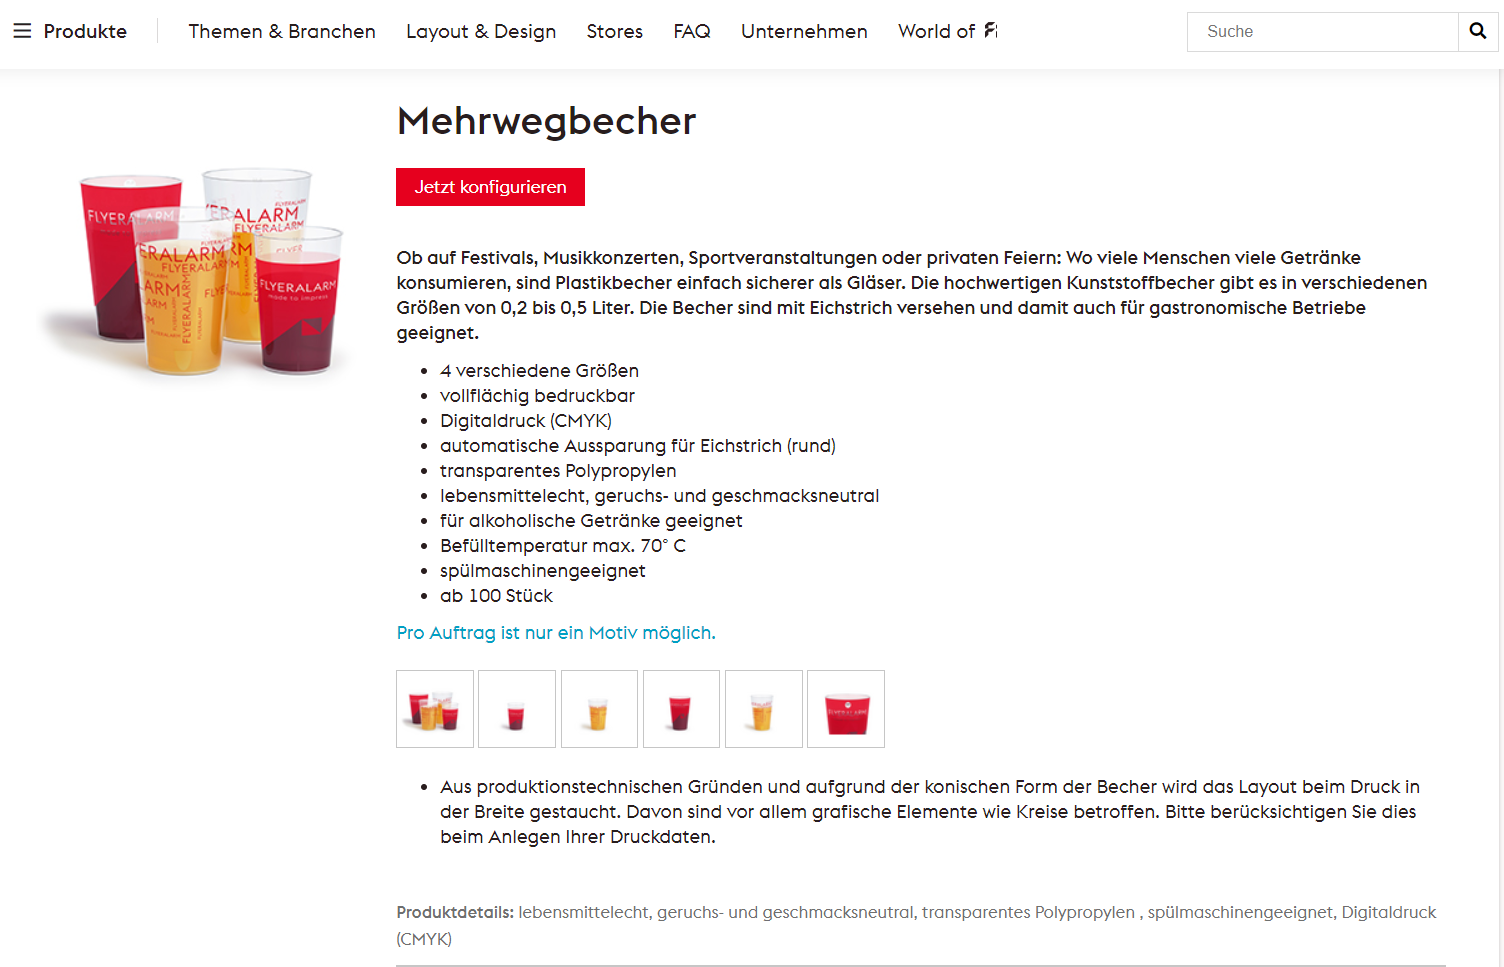
\epsfig{file = technik/images/flyeralarm.png, width=11.0cm}}
	\caption[Mehrwegbecher bestellen]{\textit{Bestellvorgang von Mehrwegbechern auf flyeralarm.com}}
	\label{fig:flyeralarm}
\end{figure}
% 
Dazu muss man, nachdem man die gewünschte Größe gewählt hat, sein Design hochladen. Dabei sollte man das Datenblatt\footnote{Das Datenblatt ist auf der Webseite zu finden und kann von dort heruntergeladen werden.} berücksichtigen, welches die Vorgaben beschreibt wie zum Beispiel Sicherheitsabstand oder Druck Farbraum. Die Online-Druckerei schreibt auf ihrer Webseite:\textit{\glqq Aus produktionstechnischen Gründen und aufgrund der konischen Form der Becher wird das Layout beim Druck in der Breite gestaucht. Davon sind vor allem grafische Elemente wie Kreise betroffen.\grqq} \cite{flyeralarm_mehrwegbecher_nodate} Eine Vorschau, wie das ganze am Ende aussehen wird, gibt es nicht. Im schlechtesten Fall hat man am Ende ein nicht zufriedenstellendes Ergebnis. Auch andere Seiten bieten ein ähnliches Angebot.Eine fertige Vorschau ist jedoch eher nicht zu finden.
%
\subsection{Spread Shirt}
\label{sec:spreadshirt}
%
Spreadshirt ist eigentlich eine Onlinedruckerei für T-Shirts. Sie selbst schreiben über sich Folgendes: \textit{\glqq Seit 2002 liefert Dir Spreadshirt T-Shirt-Druck in bester Qualität. Was als Start-up-Idee in Leipzig begann, ist inzwischen ein weltweit erfolgreiches Print-on-Demand-Unternehmen, das Wert auf faire Handels- und Produktionswege legt, seine Verantwortung als internationaler Arbeitgeber ernst nimmt und seinen Mitarbeitern ein attraktives Arbeitsumfeld bietet.\grqq } \cite{spreadshirt_tassen_nodate}
%
\begin{figure}[h]
	\centering
	{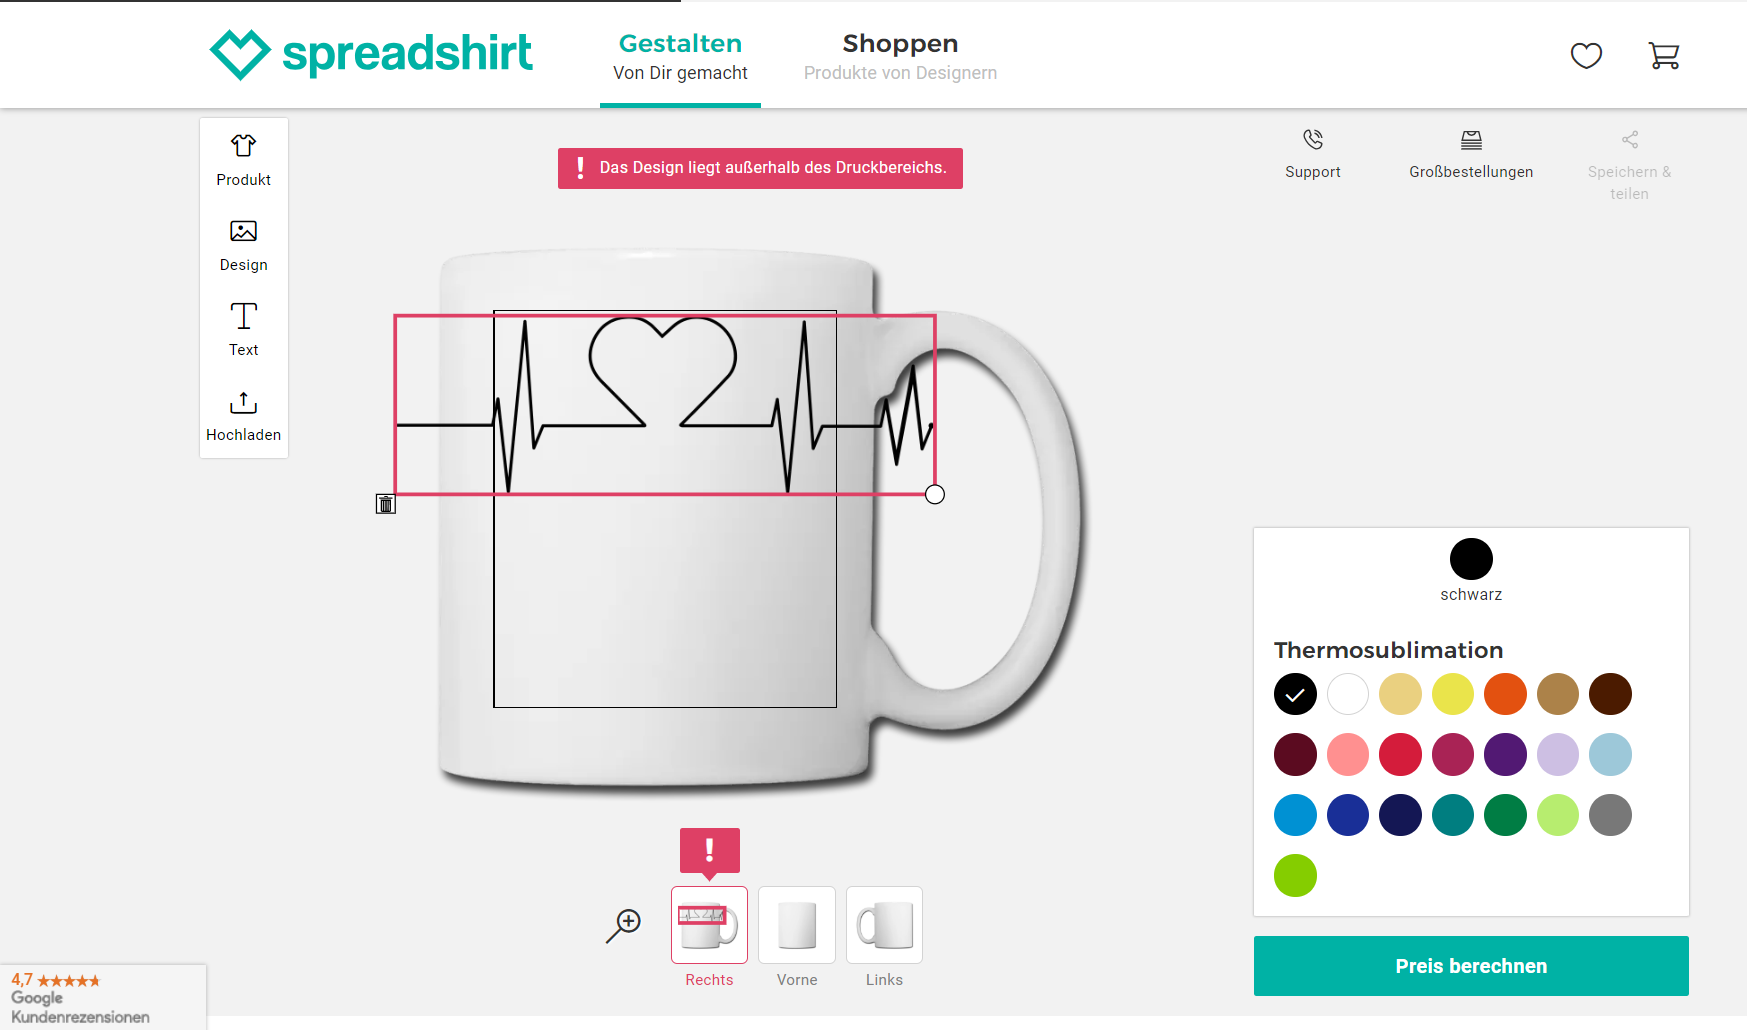
\epsfig{file = technik/images/spread-shirt.png, width=11.0cm}}
	\caption[Tasse bestellen]{\textit{Gestaltung einer Tasse auf spread-shirt.com}}
	\label{fig:spread}
\end{figure}
%
Zwar wird kein Druck von Mehrwegbechern angeboten, dafür aber der Druck von Tassen. Der Kunder kann hier in einem Online-Konfigurator seine Tasse selbst gestalten, indem er Text oder Bildelemente auf die Tasse legt. Das ganze wird sogar in 3D angezeigt. Jedoch ist die Ansicht nicht flexibel sondern statisch. Man kann die Tasse lediglich von drei verschiedenen Blickwinkeln betrachten (rechts, vorne, links). In unserem Fall sollen fertige Designs dargestellt werden. Auch das ist beim Tassenkonfigurator von Spreadshirt schwierig. Wie in der Abbildung \ref{fig:spread} zu sehen kann ein Objekt nur im Druckbereich dargestellt werden, nicht außerhalb des Bereichs. Damit ist ein Rundum-Druck nicht möglich. \\
Trotzdem lässt sich sagen, dass dieser Konfigurator gut und übersichtlich gestaltet ist. Jedoch hat er nicht die Funktionalität, welche der Konfigurator für Gizeh haben sollte.
%
\subsection{Becher-bedrucken.de}
\label{sec:currycup}
%
Ein weiteres Angebot für Becher gibt es auf \textit{becher-bedrucken.de}. Dort gibt es einen 3D Konfigurator für verschiedene Becher. Der technische Ansatz ist schon sehr gut und kann bei der Entwicklung berücksichtigt werden. Es werden ähnliche Technologien verwendet, wie in dieser Arbeit. Jedoch sind die Designvorgaben ganz anders als die Druckvorgaben von Gizeh. Das hochgeladene Design ist so angepasst, das es bestmöglich auf dem Becher angezeigt werden kann.
%
\begin{figure}[h]
	\centering
	{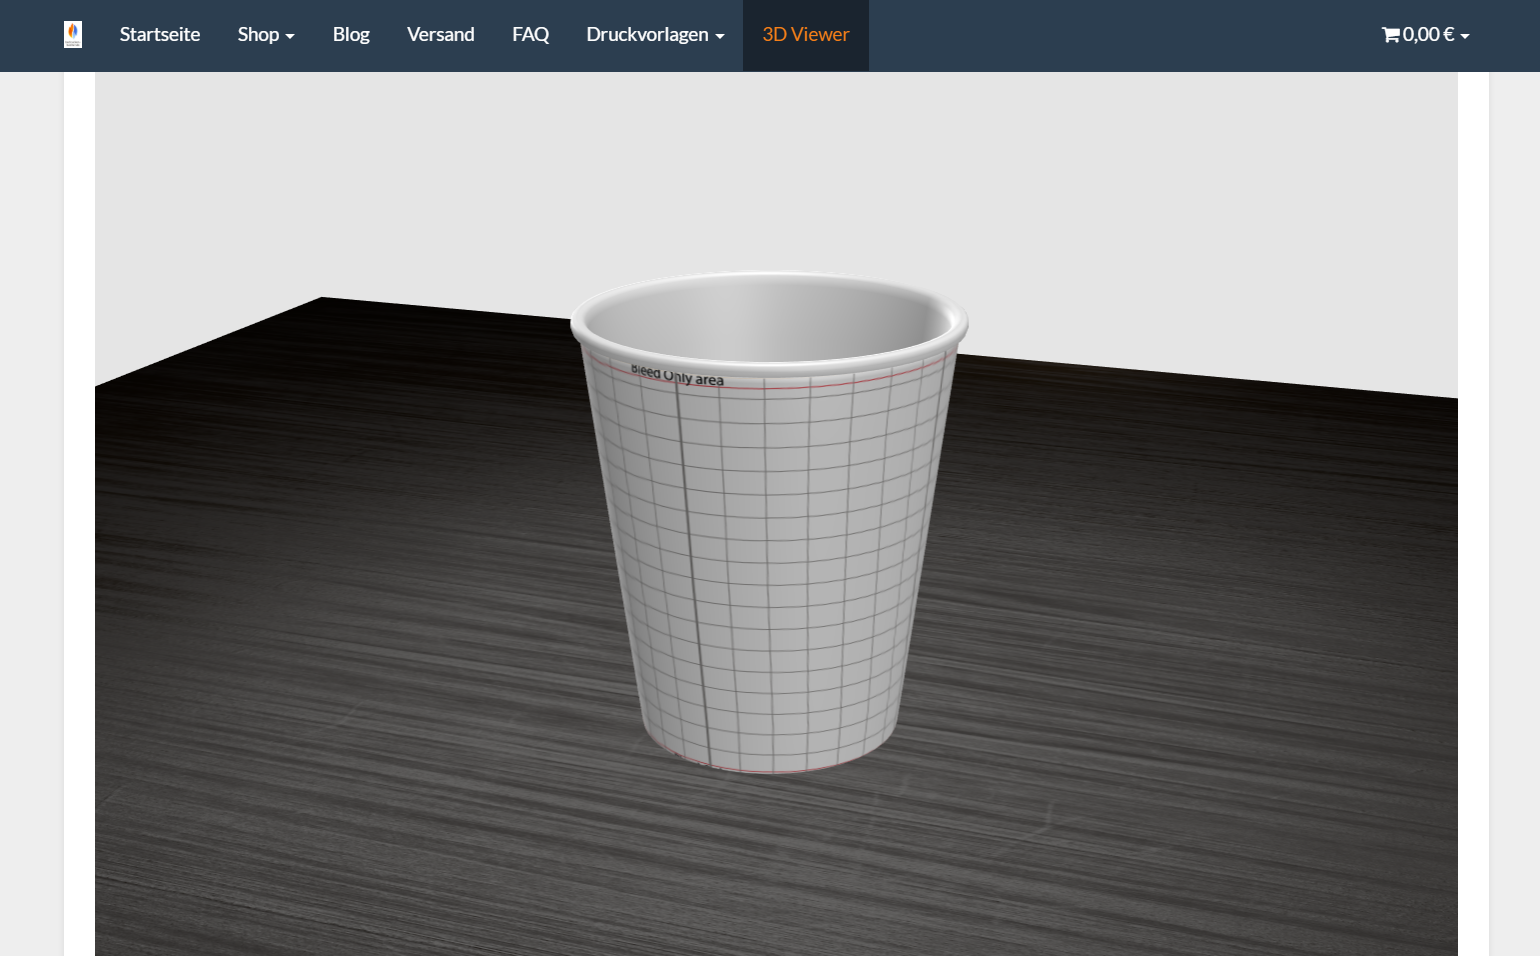
\epsfig{file = technik/images/becher-bedrucken.png, width=11.0cm}}
	\caption[Becher bedrucken]{\textit{3D Viewer eines Bechers auf bedrucken-becher.de}}
	\label{fig:becherbedrucken}
\end{figure}
%
Die Darstellung in 3D ist schön anzusehen. Zumindest auf einem Gerät mit größerem Display. Eine Anpassung für mobile Geräte ist so gut wie gar nicht vorhanden. Technisch gesehen kann aber trotzdem an diesen Lösungsansatz angeknüpft werden.
%
\section{3D Online Konfiguratoren}
\label{sec:3dconfigurators}
%
Heutzutage kann nahezu alles bedruckt werden. Die Vielzahl an Produkten ist groß. Dies haben wir bisher in diesem Kapitel erläutert, wie das konkret bei Bechern oder Tassen aussehen kann. Schwieriger zu finden sind allerdings 3D Konfiguratoren für diese Produkte. Oft gibt es höchsten eine 3D Pop-Up Ansicht, eine alte Lösung mit Flash o. ä. Eine responsive Lösung ist eher nicht zu finden. \\
In der Autoindustrie und anderen Branchen sind jedoch einige gute 3D Konfiguratoren umgesetzt. Wenn man eventuell die passenden Felgen sucht, bekommt man da einen übersichtlich gut gestalteten Konfigurator in 3D. Teilweise sind Konfiguratoren zu finden, welche responsiv sind. Einige Firmen bieten sogar an 3D Konfiguratoren für bestimmte Produkte umzusetzen. Dabei handelt es sich meist um individuelle Lösungen. Das Folgende Beispiel soll zeigen, das es durchaus möglich ist gute 3D Konfiguratoren zu entwickeln.
%
\begin{figure}[]
	\centering
	{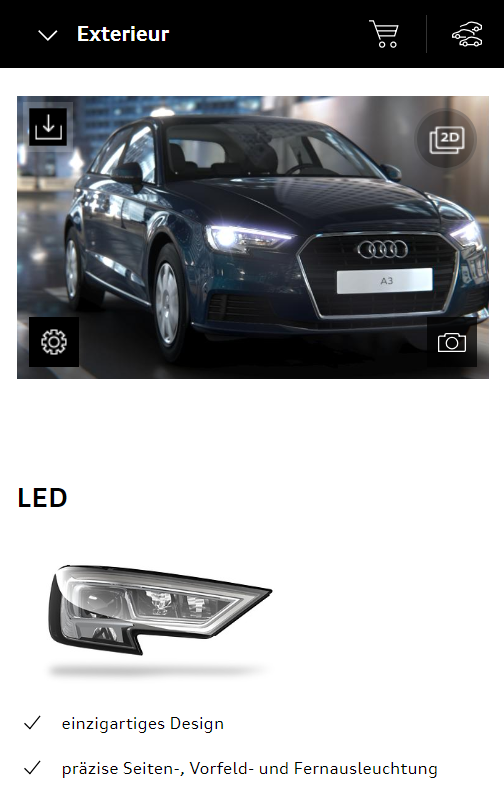
\epsfig{file = technik/images/audi.png, width=6.0cm}}
	\caption[Audi Konfigurator]{\textit{Neue 3D Ansicht von Audi}}
	\label{fig:audi}
\end{figure}
%
%
\paragraph{Audi 3D Konfigurator}Letztes Jahr veröffentlichte Audi seinen neuen Konfigurator auf der Webseite. Er rendert die Fahrzeuge in Echtzeit. Die Anwendung ist auch für mobile Geräte optimiert (siehe Abbildung \ref{fig:audi}). So kann man den Konfigurator beispielsweise mit Toucheingaben steuern. Man kann sich das Fahrzeug ganz genau anschauen und an Details heranzoomen. Technisch eine sehr gute Umsetzung, die auch optisch etwas her macht. \\
%
Bei dem 3D Konfigurator für Mehrwegbecher soll zusätzlich ein eigenes Design gerendert werden. Eine wirklich zufriedenstellende Lösung gibt es da nicht. Mit aktuellen Technologien, könnte ein Lösung umgesetzt werden. Diese sind oft noch sehr jung und wenig dokumentiert, aber haben gute Voraussetzungen um eine Lösung zu entwickeln.
%
\section{Webframeworks}
\label{sec:webframeworks}
%
Wofür es früher Flash gab, werden nun Frameworks wie \textit{Angular} oder \textit{ReactJS} verwendet. Es handelt sich dabei um Frontend Frameworks für Webapplikationen. Dabei hat man heutzutage oft die Qual der Wahl. Die Anzahl der Angebote an Frameworks und Libraries ist groß. Sie kommen oft beim Entwickeln von \textit{Single Page Applications (SPA)}  zum Einsatz.
%
\paragraph{Angular}
\label{p:angular}
%
ist nichts anderes als ein JavaScript-Framework auf Basis von TypeScript\footnote{Eine von Microsoft entwickelte Programmiersprache. TypeScript ist eine kompilierte und plattformübergreifende Sprache, die reine JavaScript-Dateien generiert.}. Es wurde von Google entwickelt und ist ein Open-Source-Framework. Es unterstützt den Entwickler dabei, moderne Webanwendungen zu machen, die zum einen für Desktop und zum andern für Mobile optimiert worden sind. Wie in der Abbildung \ref{fig:googletrends} zu sehen, ist \textit{Angular} das meist genutzte und bekannteste Framework für SPAs. Ähnliches zeigt auch die Stack Overflow Entwicklerumfrage 2018: Bei den meist genutzen Bibliotheken und Frameworks liegt Angular mit 36,9\% einen Platz vor React mit 27,8\% \cite{stackoverflow_stack_2018}.
%
\begin{figure}[h]
	\centering
	{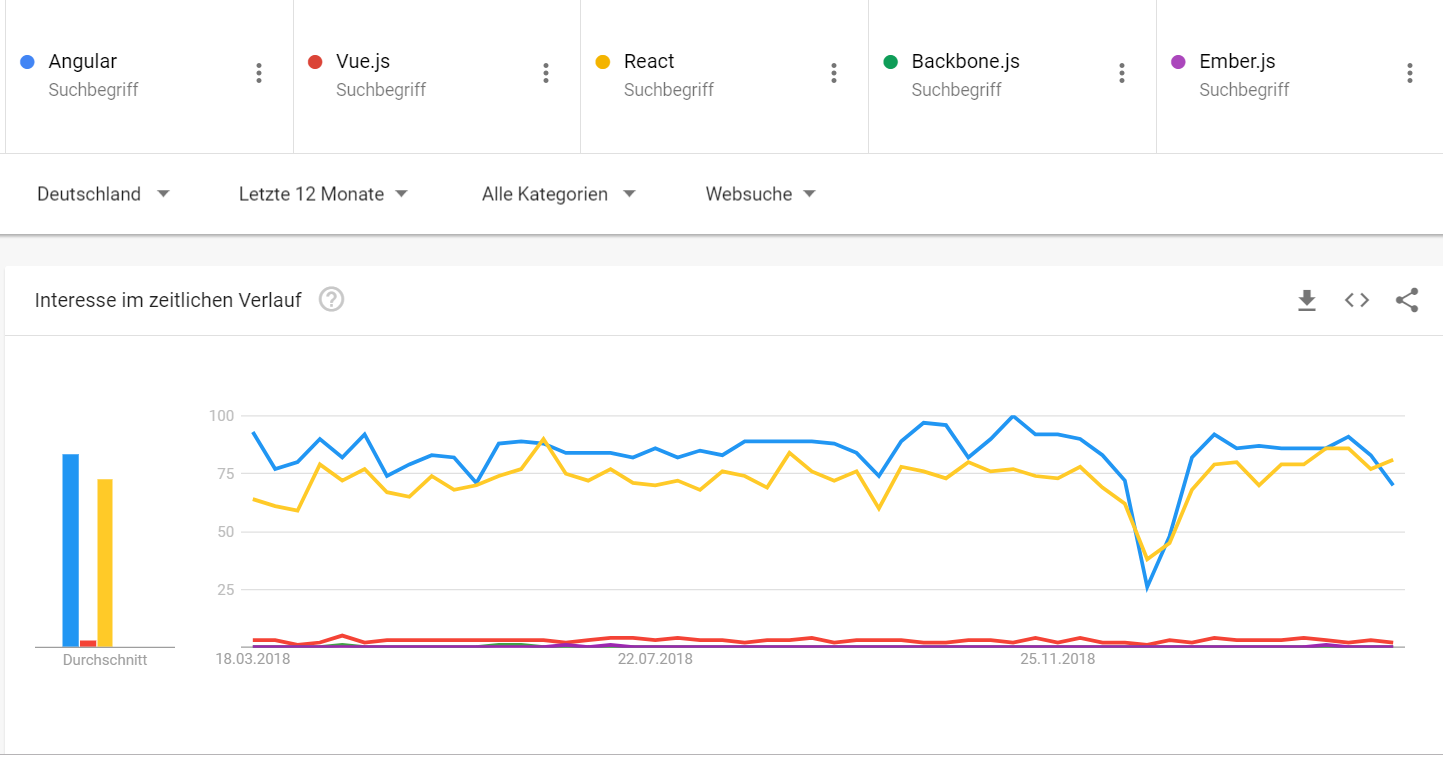
\epsfig{file = technik/images/google-trends.png, width=13.0cm}}
	\caption[Audi Konfigurator]{\textit{Google Trends Statistik. Suchanfragen von Frontend-Frameworks in 2018}}
	\label{fig:googletrends}
\end{figure}
%
Außerdem gibt es den Entwicklern Konventionen und Richtlinen an die Hand. Das ist gerade dann sinnvoll, wenn man in einem großen Team arbeitet. Oder bei großen Projekten für ein einfaches Handling und die Wartbarkeit des Codes sinnvoll wird. Ein Merkmal von Angular ist, das es viele unterschiedliche Module gibt, die es ermöglichen, sehr effizient Anwendungen zu produzieren. Da gibt es Module, welche für die Client-Server-Kommunikation zuständig sind. Sie ermöglichen die Kommunikation mit dem Backend. Ein anderes Modul ist für die Bindung der Daten zuständig. Wenn ich auf einer Ansicht Informationen bereitstellen möchte, die zum Beispiel aus einer Datenbank kommen, kann ich das ganz einfach mit dem Bindungsmechanismus von Angular umsetzen. Das Framework ist auch bekannt für seine tollen Animationen auf Basis von Web-Animation. Ein weiteres, wichtiges Modul ist das Routing-Modul. Im Grunde genommen sind Routings Grundbestandteil für \textit{Single Page Anwendungen}. Mittels Routings kann ich festlegen welcher Teil der Anwendung nun angezeigt werden soll. Außerdem baut das Framework auf die komponentenbasierte Programmierung. In Kapitel 3 werden wir noch genauer auf Angular eingehen\footnote{Die Dokumentation des Frameworks ist unter \textit{https:/angular.io/docs/} zu finden.}.
%

%
\paragraph{React}
\label{p:react}
%
ist das meistgesuchte JavaScript Framework 2018 \cite{stackoverflow_stack_2018}. Es wurde 2013 von Facebook entwickelt und viele bekannte Unternehmen wie Netflix, Twitter oder PayPal verwenden das Framework. Ähnlich wie Angular setzt React auf modulare Komponentenarchitektur. Damit wird der Frontendcode leicht nachvollziehbar. \textit{\glqq Das Ziel von React ist es, einfacheren Code schreiben zu können, dessen Bestandteile weniger miteinander verschränkt oder verwoben sind \grqq}\cite{kogel_paul_react_2015} \\
React ist kein Framework, es ist eine Bibliothek. Es ist ein sehr flexibles Werkzeug, dass in bestehende Anwendungen eingebaut werden kann, ohne den ganzen Code umzustrukturieren. Dem Entwickler wird keine Grundstruktur für seine Applikation gegeben, was ein wesentlicher Unterschied zu Angular ist. Ein weiteres Merkmal von React ist die virtuelle DOM. Diese garantiert die Synchronisierung der DOM indem bei Änderungen alles neu gerendert wird\footnote{Die vollständige Dokumentation ist unter \textit{https://reactjs.org/docs/getting-started.html} zu finden}.
%
\paragraph{Vue.js}
\label{p:vueJS}
%
ist ein weiteres Frontend-Framework zur Entwicklung von \textit{Single Page Anwendungen}. Es ist nicht das beliebteste Framework und trotzdem taucht es immer wieder auf (siehe Abbildung \ref{fig:googletrends}) und ist definitiv eine Alternative zu \textit{Angular} oder \textit{React}. Es setzt auch auf eine modulare Architektur, die in einzelne Komponenten zerteilt ist. Das Framework ist im Vergleich zu seinen Konkurrenten deutlich einfacher und hat eine flache Lernkurve. Dadurch ist es auch schneller und bringt dem Framework einen Vorteil gegenüber den Alternativen. Obwohl es kleiner ist, bringt es trotzdem alle wichtigen Funktionen wie Suchmaschinenoptimierung mit sich. Es kann auch in Kombination mit React verwendet werden. In Vue.js wird ohnehin das bekannte virtul DOM genutzt. Auch die Community ist stetig am wachsen.\footnote{Weitere Informationen sind in der offizielen Dokumentation unter \emph{https://vue.js.org/v2/guide} zu finden.} \\
%
%
%
%%%%%%%%%%%%%%%%%%%%%%%%%%%%%%%%%%%%%%%%%%%%%%%%%%%
%
% A U F B A U 
%
%%%%%%%%%%%%%%%%%%%%%%%%%%%%%%%%%%%%%%%%%%%%%%%%%%%
%
\section{Flash und WebGL}
\label{sec:webgl2}
%
In dem Artikel \emph{HTML5/WebGL vs Flash in 3D Visualisation} schreibt der Autor folgendes über WebGL:\\

\textit{\glqq Die Entwicklung verbesserter 3D-Grafiken in webbasierten Anwendungen hat in letzter Zeit einen Schritt vorwärts getan, als Programmierer WebGL in die Mozilla Firefox Nightly-Builds und in WebKit integriert haben, das in Google Chrome und dem Safari-Browser von Apple verwendet wird. WebGL ist eine der am meisten entwickelten Bibliotheken, die von HTML5 unterstützt werden.\grqq } \cite{bahor_html5/webgl_2013}.\\

Adobe Flash ist auch heute noch vielen ein Begriff. Es war darauf ausgerichtet interaktive 2D Grafiken im Web bereitzustellen. Mit der Veröffentlichung der Version 10 des Flash Players haben die Entwickler sogar eine z-Achse eingeführt. Sie ermöglicht eine 3D Darstellung und Transformation von Objekten. Diese Unterstützung für die Interaktion von Objekten der dritten Dimension wurde jedoch in begrenzter Weise bereitgestellt.\\
Einer der aktuellsten Leistungstests zwischen dem Flash- und dem WebGL-Canvas-basierten 3D-Inhalt zeigt deutlich, dass der HTML5-Canvas beginnt, höhere Frameraten zu generieren und 3D-Inhalte im Web zu rendern. Die Testergebnisse zeigen, dass WebGL beim Rendern von 3D-Inhalten wesentlich schneller abschneidet und höhere Frameraten für die 3D-Animationen im Web bietet, während sie mit Flash verglichen werden. Weiter schreibt Senad Bahor in seinem Artikel, dass \textit{es eigentlich bei der 3D-Grafik darum geht, dass 3D-Modell zu ändern und zeitabhängig zu sehen. Dies kann derzeit nur durch die Verwendung der HTML5- und WebGL-Engines im Web erreicht werden, da HTML5 Interoperabilität zwischen verschiedenen Elementen (sowohl traditionellen als auch HTML5-basierten) bietet, während JavaScript dazu veranlasst wird, die Renderprozedur durch den WebGL-Prozess zu handhaben.}\cite{bahor_html5/webgl_2013}\\
Weiter zeigen die Ergebnisse des Artikels deutlich, dass Flash-basierte 3D-Grafiken auf iOS-basierten Geräten nahezu nicht darstellbar sind, da Adobe mit seinem Flash-Plugin nie iOS unterstützt hat. Aufgrund der HTML5-Funktionalität und -Erreichbarkeit kann die Webseite auch auf einer Vielzahl von Geräten, einschließlich iOS- und Android-Geräten, wiedergegeben werden, ohne dass sich die Benutzer um das Vorhandensein der Plugins und die Versionierung des Players kümmern müssen.
Webbrowser entwickeln sich stetig weiter. WebGL kann in über 95\% aller Browser verwendet werden \cite{deveria_alexis_can_2013}. Was zuvor schon in Videopielen mit OpenGL möglich war, ist nun auch im Web möglich. Wie genau WebGL als Abstraktionsschicht für den grafischen Teil einer Anwendung verwendet werden kann, wird in Kapitel \ref{sec:javascriptbibliotheken} erläutert.

Mit WebGL müssen die Benutzer nicht dazu aufgefordert werden, eines der Plugins zu installieren, um den 3D-Inhalt auf der Website zum Laufen zu bringen. Die einzige Voraussetzung ist, dass der Webbrowser das HTML5-Canvas-Element unterstützt, über das WebGL den Inhalt für den Benutzer darstellt.\\
Im Wesentlichen kann WebGL auf jeder Plattform und auf allen großen Systemen mit OpenGL-fähiger Grafikkarte und einem Browser ausgeführt werden, der WebGL unterstützt.\\

\section{3D JavaScript Bibliotheken}
\label{sec:javascriptbibliotheken}
%
Um eine 3D Szene mit WebGL darzustellen wird ein JavaScript Framework benötigt. Es erstellt und rendert eine Szene mit den 3D Objekten. Im Folgenden werden die zwei bekanntesten und weit verbreitetsten Bibliotheken vorgestellt.
\paragraph{ThreeJS}
\label{sec:threeJS}
%
\textit{Three.js} ist es eine sehr seriöse WebGL-Bibliothek mit einer starken Community und vielen guten Beispielen. Es wird auch oft in kommerziellen Webanwendungen verwendet. Die erste Version des Frameworks tauchte 2010 auf und der Quellcode wird in einem Repository auf GitHub gehostet\footnote{https://github.com/mrdoob/three.js/}. Three.js hat eine verständliche Struktur und große Anpassungsmöglichkeiten. Es ist eine Anwendungsprogrammierschnittstelle, mit der animierte 3D-Grafiken in einem Webbrowser erstellt und angezeigt werden. Neben der Dokumentation gibt es auch ein Wiki, was dem Entwickler zum schnellen Einstieg sehr helfen kann\footnote{https://github.com/mrdoob/Three.js/wiki/}.Schon beim erstellen einer einfachen Szene mit dem Framework fällt auf, das es dem Prinzip der objektorientierten Programmierung folgt\footnote{https://threejs.org/docs/\#manual/en/introduction/Creating-a-scene}. In dem Kapitel \ref{cha:introduction} wird noch genauer auf das Framework eingegangen.
%
%\begin{figure}[h]
%	\centering
%	{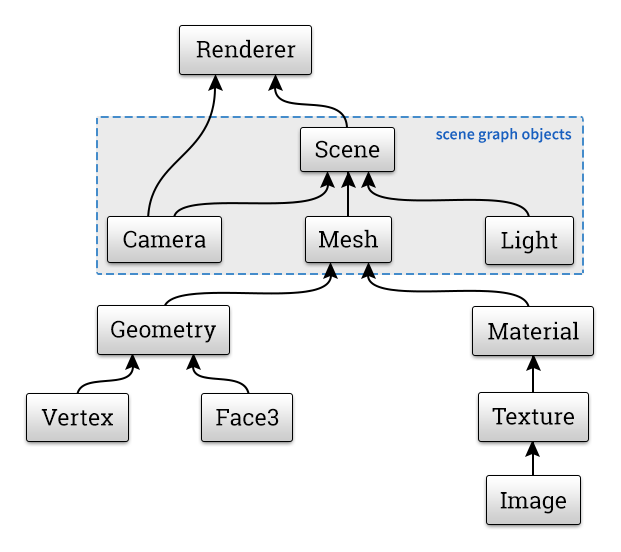
\epsfig{file = technik/images/node-map.png, width=11.0cm}}
%	\caption[Audi Konfigurator]{\textit{Aufbau einer Szene in Three.js}}
%	\label{fig:threejs}
%\end{figure}
%
%
\paragraph{BabylonJS}
\label{sec:babylonJS}
%
Babylon.js\footnote{Die offizielle Dokumentation ist unter \textit{https://doc.babylonjs.com/} zu finden.} ist ein Framework, mit dem komplette 3D-Webanwendungen erstellen werden können. Babylon.js hat eine Community, die stetig wächst und auch aktiv zum Projekt beiträgt und immer mehr Funktionen hinzufügt. Das Framework hat alle notwendigen Werkzeuge, um 3D-Anwendungen umzusetzen. Sie können 3D-Objekte laden und zeichnen, diese 3D-Objekte verwalten, Spezialeffekte erstellen und verwalten, räumliche Sounds spielen und verwalten, Gameplay erstellen und vieles mehr. 
%
\begin{figure}[h]
	\centering
	{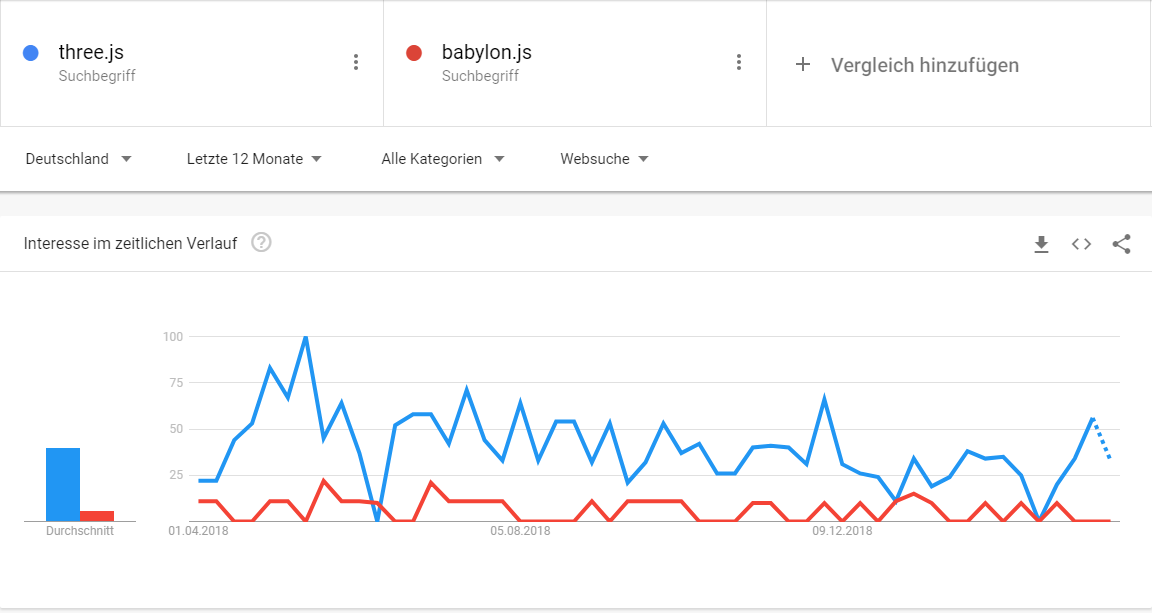
\epsfig{file = technik/images/3d-framework.png, width=13.0cm}}
	\caption[Audi Konfigurator]{\textit{Google Trends: Vergleich Three.js und Babylon.js in den letzten 12 Montaten}}
	\label{fig:compare3dframework}
\end{figure}
%
Babylons.js ist ein benutzerfreundliches Framework, da Sie diese Dinge mit den minimalen Codezeilen einrichten können. Es ist ein mit TypeScript entwickeltes JavaScript-Framework. \cite{moreau-mathis_babylon.js_2016} Wie in Abbildung \ref{fig:compare3dframework} zu sehen ist Babylon.js jedoch weniger gefragt als three.js. Das zeigt sich auch in den 3D Webanwendungen, wo auch meist three.js verwendet wird.

		
		%---- Kapitel Grundlagen ----
		%
%%%%%%%%%%%%%%%%%%%%%%%%%%%%%%%%%%%%%%%%%%%%%%%%%%%
%
%  E N T W I C K L U N G S U M G E B U N G
%
%%%%%%%%%%%%%%%%%%%%%%%%%%%%%%%%%%%%%%%%%%%%%%%%%%%
\chapter{Grundlagen}
\label{cha:grundlagen}
%
%
In dem Grundlagenkapitel geht es um das Basiswissen, auf dem die Arbeit aufbaut. Es wird näher auf die verwendeten Technologien eingegangen. Dabei werden die Frontend-Frameworks beleuchtet sowie die 3D Bibliotheken. Näher wir auch auf die Begriffe Resposive Webdesign, Usability und Performance eingegangen.
%
%
%%%%%%%%%%%%%%%%%%%%%%%%%%%%%%%%%%%%%%%%%%%%%%%%%%%
%
% S P A
%
%%%%%%%%%%%%%%%%%%%%%%%%%%%%%%%%%%%%%%%%%%%%%%%%%%%
%
\section{Single Page Anwendungen}
\label{sec:spa}
%
Früher war es bei Webanwendungen wichtig, soviel wie möglich auf dem Server zu erledigen. Bei modernen Webframeworks gilt jedoch genau das Gegenteil. Es wird versucht möglichst viel clientseitig umzusetzten.\textit{\glqq Dies steigert die Benutzerfreundlichkeit und schafft die Möglichkeit der Anpassung an die Auflösungen und Formfaktoren der vielen unterschiedlichen klassischen und mobilen Plattformen.\grqq } \cite{bahor_html5/webgl_2013}. Im Folgenden wird nun kurz etwas genauer darauf eingegangen was André Krämer in seinem Videokurs sehr gut und einfach erklärt hat.
%
\paragraph{Klassische Webanwendungen}
%
Bevor man sich damit befasst was Single Page Anwendungen sind, sollte man sich das Prinzip einer klassischen Webanwendung anschauen. Nehmen wir beispielsweise an, ein Client sendet eine Anfrage an einen Server. Hierbei handelt es sich um einen Webbrowser, welcher eine Webadresse öffnen möchte. Der Zielserver übernimmt die Verarbeitung. In der Regel laufen nun Skripte auf dem Server, welche HTML rendern. Schließlich bekommt der Client auf seine Anfrage eine Antwort in Form eines HTML-Dokumentes und kann es dann anzeigen. Bei diesem Vorgang liegt die komplette Verarbeitung bei dem Server. Der Webbrowser dient lediglich der Darstellung und einfachen Eingabe. Das die Daten auf einem Server verarbeitet werden wird deutlich, wenn ein Seitenwechsel vorgenommen wird. Dabei wird kurze Zeit nichts angezeigt während die Seite komplett neu lädt.\\
Mit der Einführung von AJAX\footnote{Ajax bzw. AJAX steht als Akronym für „Asynchronous JavaScript and XML“. Die Technologie ermöglicht es, einzelne Teile einer Webseite bei Bedarf asynchron zu laden, so dass sie dynamisch wird. Der angezeigte Inhalt lässt sich gezielt so manipulieren, ohne die komplette Seite neu zu laden.} in 2005 machte die Webentwicklung einen Schritt nach vorne. Nun war es nämlich möglich, Daten asynchron an den Server zu senden. Das heißt, der Server verabreitet zwar immer noch die Daten, sendet nun aber nur noch einen Teil des vorgerenderten Dokuments oder sogar nur einzelne Daten der Seite. Somit wird die Seite nicht wieder komplett neu geladen. Wenn man nun aber in einen komplett andern Bereich der Seite wechseln will, hilft AJAX nicht. Die Seite wird neu geladen und es dauert einen kurzen Moment bis das Ergebnis vom Webbrowser angezeigt werden kann. Um dieses Problem zu lösen, kommen \textit{Single Page Anwendungen} zum Einsatz.
\paragraph{Dezentralisierung der Webanwendung}
%
Im Grunde arbeiten SPA's nach folgendem Prinzip: Der Webbrowser sendet eine Anfrage an den Server. Dieser verarbeitet, wie bei klassischen Webanwendungen nun die Anfrage. Anschließend wird im Webbrowser eine Benutzeroberfläche dargestellt. Nun kommt der entscheidende Unterschied zu klassischen Anwendungen. Bei einem Seitenwechsel oder anderen Interaktionen des Benutzers wird eine neue Benutzeroberfläche erzeugt, indem Teile der Seite ausgetauscht werden. Die Seite wird nie komplett neu geladen. Der Nutzer bleibt immer auf der einen Seite, zumindest fühlt es sich für den Benutzer so an. Dieses Prinzip kennt der Anwender von Desktop-Anwendungen. Man hat sogar die Möglichkeit die Anwendung (zumindest teilweise) offlinefähig zu machen.\\
Die Grundlage einer solchen Anwendung ist das Routing. Abhängig vom Pfad werden bestimmte Bausteine der Anwendung angezeigt bzw. ausgeblendet. Wie wir im späteren Verlauf dieser Arbeit noch sehen werden, hat man tatsächlich nur eine HTML-Datei, welche abhängig vom Kontext immer andere Inhalte anzeigen kann.\\
%
Zusammenfassend lässt sich also festhalten, das ein Ziel von SPAs ist, die Kommunikation zwischen Client und Server enorm zu reduzieren. Um dies zu erreichen wird die Anwendung dezentralisiert. Das heißt, es gibt nur ein HTML Dokument\cite{domin_was_2018}. Durch den Einsatz von Frameworks, wie Angular, ist es möglich Inhalte zu aktualisieren oder zu einer anderen Seite zu wechseln, ohne die Seite über den Server neu zu laden.
\footnote{Das Prinzip von Single Page Anwendungen wird zum Beispiel von Googles Gmail und Gmaps sowie von Twitter verwendet}
%
%
%%%%%%%%%%%%%%%%%%%%%%%%%%%%%%%%%%%%%%%%%%%%%%%%%%%
%
% A U F B A U 
%
%%%%%%%%%%%%%%%%%%%%%%%%%%%%%%%%%%%%%%%%%%%%%%%%%%%
%
\section{Framework Angular}
\label{sec:angular7}
Das Framework Angular ist sehr umfangreich. Im Folgenden werden einige Grundlagen erläutert, die zur Implementierung einer Anwendung mit Angular benötigt werden. Dabei soll ein Grundverständis vermittelt werden, wie das Framework aufgebaut ist und wie es arbeitet.
\subsection{Komponentenbasierte Programmierung}
%
Angular ist ein Framework, das auf Komponenten setzt. Das Prinzip der komponentenbasierten Entwicklung kommt nicht nur bei Angular vor, sondern auch bei vielen anderen Programmiersprachen und Frameworks. Was in Angular Komponenten sind wird in dem Buch \textit{Angular: Grundlagen, fortgeschrittene Techniken und Best Practices mit TypeScript - ab Angular 4, inklusive NativeScript und Redux} folgendermaßen beschrieben:\\
%

\textit{\glqq Komponenten sind die Grundbausteine einer Angular Anwendung. Jede Anwendung ist aus vielen verschiedenen Komponenten zusammengesetzt, die jeweils eine bestimmte Aufgabe erfüllen. Eine Komponente beschreibt somit immer einen kleinen Teil der Anwendung, z. B. eine Seite oder ein einzelnes UI-Element.\grqq }\cite{woiwode_angular:_2017} \\

%
Im Grunde ist eine Komponente also nichts anderes als ein selbstdefinierter HTML-Knoten, den man im HTML Kontext ganz normal nutzen kann. Man erzeugt einfach DOM-Elemente\footnote{Wenn eine Webseite geladen wird, erstellt der Browser eine Document Object Model der Seite. Das HTML-DOM-Modell ist als Baum von Objekten aufgebaut. Diese Objekte sind ein der Regel einfache HTML-Tags} und kann sie dann automatisch in Angular nutzen.
Eine Komponente in Angular ist in drei Parts aufgeteilt: Logik, Vorlage und Style. Die Logik beschreibt die TypeScript Klassen, Eigenschaften, Methoden und so weiter. Sie beschreibt also, was zu tun ist, wenn zum Beispiel ein bestimmter Button geklickt wird. Die Vorlage (Template) ist ein HTML-Schnipsel. Dies kann einfach nur ein Button-Element sein oder auch eine HTML-Struktur mit mehreren HTML-Elementen. Sie beschreibt die Stuktur bzw. den Aufbau der Komponente. Wie die Komponente aussehen soll wird in dem Style Part festgelegt. Dabei ist zu beachten, dass die Style-Definitionen nur innerhalb der Komponente gelten. Globale Styles der Anwendung werden seperat definiert.\\
Der Startpunkt der Anwendung ist die \texttt{index.html}. Sie definiert die Applikationskomponente, der Ankerpunkt einer Angular-Anwendung, quasi eine Basiskomponente. In Dieser können nun weitere Kindskomponenten eingefügt werden, welche auch ineinander verschachtelt sein können. So entsteht eine komplette Struktur. Eine Komponentenvorlage kann also nicht nur HTML-Elemente enthalten, sondern auch Kindskomponenten. Entscheidend ist, das Komponenten verschachtelt werden können. Dies ist das Grundprinzip der komponentenbasierten Programmierung (vgl. Angular Grundkurs\cite{unlu_angular_2018}).

\subsection{Modulare Umsetzung}
Schauen wir uns nun an, wie Angular mit Modulen arbeitet und was genau Module sind. \textit{Nikolas Poniros} hat das in seinem Buch \textit{Angular für Dummies} so definiert:\\

\textit{\glqq Angular-Module helfen beim Gliedern einer Webanwendung in verschiednene Funktionsblöcke. Alle Angular-Bausteine, die logisch zu einem Funktionsblock gehören, werden mit dem entsprechenden Angular-Modul registriert. Die registrierten Bausteine gehören dann zum Angular-Modul. Angular-Module sind von der Denkweise her vergleichbar mit ECMA-Script-Modulen. ECMA-Script-Module kapseln TypeScript-Konstrukte wie Klassen und Funktionen und erlauben nur den Zugriff auf exportierte Konstrukte. Angular-Module kapseln Komponenten, Pipes und Direktiven\footnote{Was genau es mit diesen Angular Bausteinen auf sich hat wird in Punkt \ref{subsec:grundfunktionen} beleuchtet.}. Ein anderes Angular-Modul kann nur auf einen Baustein zugreifen. wenn es dieses exportiert.\grqq \cite{poniros_angular_2019} }\\

Angular bietet also die Möglichkeit modular zu arbeiten. Die einzelnen Elemente und Funktionalitäten können in Modulen gruppiert werden. Im Grunde ist ein Modul nichts anderes als ein Container. Sie lassen sich besonders gut verwenden, wenn man mit mehreren Entwicklern zusammenarbeiten möchte. Module sind einzelne Bestandteile der Anwendung und lassen sich ganz einfach in bestehende Anwendungen einbauen. So kann ich ein Modul in mehreren Anwendungen wiederverwenden. Oder verschiedene Teammitglieder entwickeln jeweils ihre eigenen Module, welche anschließend in einer Anwendung zusammengefügt werden können. Ich kann ein Modul also auch in einem anderen Kontext wiederverwenden. Ein Modul darf allerdings nur in einem einzigen Modul initialisiert werden. Stattdessen wird das Modul bei mehrfacher Verwendung lediglich importiert. Folgendes Beispiel soll das Prinzip modularer Umsetzung verdeutlichen.\\
%
\begin{figure}[h]
	\centering
	{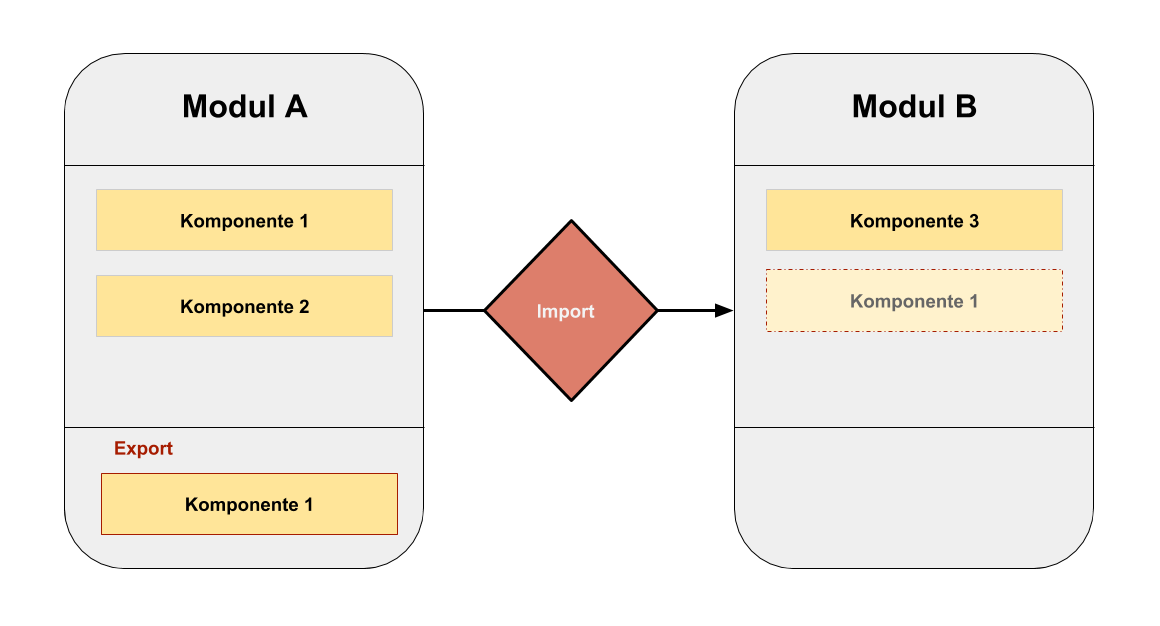
\epsfig{file = grundlagen/images/module.png, width=14.0cm}}
	\caption[Audi Konfigurator]{\textit{Fallbeispiel mit zwei Angular Modulen mit Komponenten}}
	\label{fig:ngModule}
\end{figure} 

%
Das hier beschriebene Beispiel ist in Abbildung \ref{fig:ngModule} zu sehen. Angenommen wir haben ein \textit{Modul A}. In diesem Modul sind nun \textit{Komponente 1} und \textit{Komponente 2} deklariert. Das heißt, es ist möglich in \textit{Komponente 1} die \textit{Kompontente 2} zu verwenden und umgekehrt, weil beide in dem \textit{Modul A} registriert sind. Jetzt haben wir ein weiteres \textit{Modul B}. In diesem ist die \textit{Komponente 3} registriert. Nun wäre es sehr praktisch, wenn \textit{Komponente 3} ebenfalls \textit{Komponente 1} aus dem anderen Modul verwenden könnte. Wie schon erwähnt darf ein Baustein in Angular nur in einem Modul registriert bzw. inititalisiert werden. Deshalb muss das \textit{Modul A} in \textit{Modul B} importiert werden, damit auch dort die \textit{Komponente 1} verwendet werden kann. Zusätzlich muss in \textit{Modul A} die \textit{Komponente 1} exportiert werden. Dadurch wird sie erst von außen frei zugänglich und somit in Bausteinen anderer Module nutzbar.
%
\paragraph{Hauseigene Module}
Angular hat auch ein paar hauseigene Module, die je nach Anwendungsfall importiert werden können. Das \textit{BrowserModule} wird für Web-Anwendungen im Angular-Umfeld genutzt und verfügt über alle Funktionalitäten, mit dem wir in der Lage sind, Ereignisse innerhalb des Browsers abzufangen, DOM-Rendering durchführen zu können und damit schließlich die lauffähige Angular-Anwendung im Browser realisieren zu können.\\
Das \textit{CommonModule} beinhaltet allgemeine Funktionen, die sehr, sehr häufig genutzt werden. Diese Funktionen liegen in Form von Direktiven und Pipes vor, womit ich bestimmen kann, ob ein HTML-Knoten angezeigt wird oder nicht oder auch Pipes, womit ich Ausgaben formatieren kann. Auch sprachabhängige Funktionalitäten sind in den \textit{CommonModule} enhalten.\\
Das \textit{HttpModule} ist dafür da, Client-Server-Kommunikation zu betreiben. Das heißt, HTTP-Requests lassen sich mit Hilfe des \textit{HttpModules} hervorragend realisieren, dafür werden Services zur Verfügung gestellt. Das \textit{HttpModule} hat auch Services für Testings und Co. Für Formulare gibt es entweder das FormsModule oder das \textit{ReactiveFormsModule}. Das hängt so ein wenig davon ab, wie man Formulare in der Anwendung gestalten will.\\
Das \textit{RouterModule} ist dafür da, um Komponenten-Routing zu realisieren. Das Routing ist die Grundlage für \textit{Single-Page-Applications}. Das heißt, über das Routing kann man bestimmen, welche Komponente dargestellt werden muss, wenn ein bestimmter Pfad in der Anwendung besucht wird.
%
\subsection{Grundfunktionen des Frameworks}
\label{subsec:grundfunktionen}
%
Module und Komponenten in Angular haben wir nun schon etwas ausführlicher betrachtet. Nun wollen wir uns weitere Funktionen und Bestandteile von Angular anschauen\footnote{Auf die weiteren Bestandteile von Angular wird hier nicht im Details eingegangen. Genauere Dokumentationen dazu sind online unter angular.io zu finden.}. Wie die einzelnen Bausteine umgesetzt und implementiert werden können sehen wir noch in Kapitel 4 Methodik am Fallbeispiel des 3D Konfigurators für Mehrwegbecher.
%
\paragraph{Bindungen}
%
\textit{\glqq Bindungen sind im Wesentlichen die Brücke zwischen der Darstellungsschicht und der Logikschicht\grqq } \cite{unlu_angular_2018}. Man kann beispielsweise Variablen oder Eigenschaften aus TypeScript-Klassen in  Vorlagen binden. Angenommen in der TypeScript-Klasse einer Komponente ist die Variable \texttt{title} deklariert. Um \texttt{title} nun in der Vorlage zu binden, schreibt man Folgendes: \texttt{ <h1> \{\{title\}\} </h1>}. Natürlich geht das ganze noch deutlich komplexer. Dadurch wird die Komponente mit ihrem Content dynamisch.
%
\paragraph{Direktiven}
%
Direktiven sind ein wichtiger Bestandteil von Angular. Direktiven werden in Vorlagen genutzt, indem ich sie als Attribute auszeichne. Das heißt, Direktiven sind oft Attribute, die in ein HTML-Element hinzugefügt werden oder auch beispielsweise dadurch deklariert, dass an ein bestimmtes HTML-Element ein bestimmtes Attribut angehängt sein muss. Attribut-Direktiven machen eigentlich nichts anderes als eine Anpassung des Aussehens beziehungsweise eine Anpassung des Verhaltens eines Elements, das heißt, es manipuliert ein vorhandenes Element im Wesentlichen.\\
Analog dazu kann man auch strukturelle Direktiven benutzen. Das gibt es zum Beispiel \texttt{ngFor}, diese ist sehr praktisch bei der Entwicklung einer Angular-Anwendung. Sie benutzt nämlich das Element, auf das sie angewendet wurde, als Vorlage, iteriert durch eine Liste, zum Beispiel ein \texttt{<ul>}-Element, und packt diese Vorlage so oft in den DOM hinein, wie es Elemente in der Liste gibt.
%
\paragraph{Pipes}
%
Angular bietet uns die Möglichkeit zur Nutzung von Pipes. Sie dienen dazu, eine Ausgabe zu manipulieren. Überwiegend werden Pipes in Vorlagen genutzt.\\
Die Pipe manipuliert die Ausgabe und sorgt dafür, dass beispielsweise der Name in Großbuchstaben (uppercase) dargestellt wird. Analog lassen sich auch Pipes in Kette schalten. Das heißt, wenn man eine Ausgabe hat, kann man diese wiederum in andere Pipes hineinpacken.
%
\paragraph{Services}
%
Der Begriff Services in der Entwicklung ist breit gefächert. Jede Programmiersprache versteht unter Services in gewissen Maßen etwas anderes. In der Angular-Welt sind Services Logiken, die nicht abhängig von der View sind. Eine Komponente besteht aus Logik- und Darstellungsschicht. In der Logikschicht ist ganz explizit eine Logik vorhanden, die nur für diese eine Komponente da ist.\\
Ein Service selber hat auch Logiken, die aber nicht allein für eine Komponente gelten, sondern auch im Kontext in anderen Bausteine genutzt werden können. Ein einfaches Beispiel dafür: Client-Server-Kommunikation. Es ist möglich einen Service zu erstellen, der das gesamte Handling des Logins steuert. Dieser Service verarbeitet dann via Passwort und Username die Client-Server-Kommunikation für das Login und empfängt vom Server dann das User-Objekt. An der anderer Stelle kann es sein, dass ich zum Beispiel die Authentifizierung überprüfen möchte oder einfach nur den Namen des Users brauche. In diesem Fall würde man den gleichen Service in der anderen Komponente wieder nutzen und könnte dann entsprechend auf die Eigenschaften des Services zurückgreifen, die es zuvor schon geholt hat.
%
\subsection{Angular CLI}
Die Angular CLI ist ein mächtiges Tool. Wie der Name schon sagt wird es über die Command Line gesteuert. Sie kann beispielsweise verwendet werden, um ein neues Angular-Projekt anzulegen. Die CLI legt dann im Hintergrund die benötigte Projektstruktur mit allen benötigten Dateien in dem gewünschten Verzeichnis ab. Anschließend ist die Anwendung sogar schon lauffähig. Man kann sie ganz bequem über die CLI starten, dabei wird standardmäßig der Developing-Server verwendet. Mit Webpack wird das ganze Projekt gebündelt. Eine sehr große Hilfe können die Code Generatoren sein. Sie erzeugen automatisch Komponenten, Module oder Services. Dabei werden automatisch alle \texttt{@import-}Anweisungen, Exports und so weiter vorgenommen. Wie das ganze konkret aussieht schauen wir uns bei der Umsetzung des Konfigurators noch einmal an. Angular bietet eine sehr gut verwendbare Testumgebung. Mit verschiedenen Modulen kann die Anwendung bis ins kleinste Detail getestet werden. Ganze User-Interaktionen können simuliert werden, auch auf verschiedenen Geräte-Klassifikationen. Wenn man die Anwendung veröffentlichen will, bietet das Framework über seine CLI eine build Funktion. Diese ermöglicht eine einfache und kompakte Lösung. Alles in allem ist Angular CLI ein sehr komfortables Tool, was einem das Erstellen einer Angular-Anwendung leichter macht.
%
\subsection{Versionen}
Das Framework Angular setzt auf das System der semantischen Versionierung (\textit{SEMVER}). Die erste Version des Frameworks war \textit{AngularJS}. Schon die erste Version hatte das Ziel, ein strukturiertes und übersichtliches Framework zu sein. Mit der \textit{Version 2} wechselte die Programmiersprache von JavaScript zu TypeScript, welches von Microsoft entwickelt wurde. Das Framework wurde mit der Version 2 also komplett neu entwickelt. Es setzt aber großteils auf das alte Konzept von \textit{AngularJS}. Da das Router-Modul schon die Version 3 hatte, wurde die nächste Version von Angular komplett auf \textit{Version 4} angehoben, damit nun wieder alle Module auf der selben Version sind \cite{bohm_robin_angular_2017}. Mittlerweile ist die aktuelle Version des Framework \textit{Angular 7\footnote{Stand März 2019}}. Die aktuelle Version bringt ein paar Bugfixes mit sich sowie mehr Flexibilität. So können beispielsweise über die \textit{Angular CLI} ganz bequem alle Pakete automatisch aktualisiert werden. Anschließend sollte das Projekt mit der neuen Angular Version lauffähig sein (siehe \cite{steyer_ruhe_2018}).
%
%
%%%%%%%%%%%%%%%%%%%%%%%%%%%%%%%%%%%%%%%%%%%%%%%%%%%
%
% A U F B A U 
%
%%%%%%%%%%%%%%%%%%%%%%%%%%%%%%%%%%%%%%%%%%%%%%%%%%%
%
\section{Three.js}
\label{sec:three.js}
%
Schon 2010 begann Ricardo Cabello Miguel die 3D-Bibliothek Three.js zu entwickeln. Mittlerweile ist er unter dem Namen Mr.doob bekannt. Als dann WebGL veröffentlicht wurde, portierte er \textit{Three.js}, um es mit der neuen Technologie zu verwenden. Mr.doob bezeichnete es als \glqq einfach zu implementieren\grqq. Er hatte damals bereits zwei andere Renderer damit gebaut. Seit dieser Zeit hat Three.js an Leistung und Raffinesse zugenommen. Nun ist es zur beliebtesten Wahl für die Erstellung von 3D-Anwendungen mit WebGL geworden. \\
Three.js abstrahiert den Kontext von WebGL und stellt die 3D-Szene als Meshes, Materials und Lightings dar \footnote{Das sind typische Bestandteile einer 3D-Szene die Grafik Programmierer kennen}. Aber Three.js ist mehr als nur eine Abstraktionsschicht für WebGL. Die Three.js-API wurde einfach konzipiert, sodass ein schneller Einstieg möglich ist. Funktionen können ziemlich einfach hinzugefügt und Three.js angepasst werden. Vordefinierte Objekte und Beispiele ermöglichen die Entwicklung von Modellierungsanwendungen bis hin zu Spielen. Auch Animationen sind einfach zu implementieren sowie Interaktionen in der Szene. Neben den Grundfunktionen der Bibliothek gibt es zahlreiche Beispiele und Extras, welche in eigene Projekte eingebunden werden können. Außerdem wurde Three.js so umgesetzt, dass eine hohe Leistung ohne Beeinträchtigung der Usability gewährleistet ist. Zudem gibt es umfangreiche Fehlerprüfungen, Ausnahmen und Konsolenwarnungen, um den Entwickler zu unterstützen.
%
\subsection{Die Szene}
\label{subsec:scene}
%
Die 3D-Bibliothek ist objektorientiert. Das heißt, Programmierer arbeiten mit JavaScript-Objekten, anstatt nur JavaScript-Funktionsaufrufe durchzuführen. Folgendes einfaches Beispiel, zeigt wie eine Szene in Three.js erstellt werden kann. \\

\texttt{var scene = new THREE.Scene();} 
\\

Über verschiedene Funktionen können dann die weiteren Bestandteile einer Szene hinzugefügt werden und anschließend mit dem Renderer gerendert werden. Da Angular auf TypeScript basiert, muss man bei der Implementierung einer Szene in Angular ein paar Dinge beachten. Diese werden in Kapitel 4 genauer erläutert. In diesem Teil werden zunächst die wesentlichen Bestandteile der Three.js Szene vorgestellt. Differenzierte Erklärungen zu Three.js sind in der offiziellen Dokumentation zu finden \footnote{http://threejs.org/docs}.
%
\paragraph{Kamera}
Es gibt verschiedene Kameratypen. Normalerweise wird immer die \textit{PerspectiveCamera} verwendet. Deshalb wird in dieser Arbeit nicht weiter auf die anderen Typen eingegangen. Die Kamera wird auch als Objekt in der Szene angelegt. Dabei müssen verschiedene Eigenschaften wie Seitenverhältnis und Position der Kamera angegeben werden.
%
\paragraph{Renderer}
Damit eine Szene gerendert werden kann, wird der Renderer benötigt. Hierbei handelt es sich schlichtweg um einen WebGL-Renderer. Der wird dann in ein \texttt{<canvas>}-Element eingefügt um die Szene darin darzustellen.
%
\paragraph{Lighting}
Damit Objekte der Szene sichtbar werden, muss ein \textit{light} oder sogar mehrere hinzugefügt werden. Sonst ist die Szene einfach nur schwarz. Three.js hat verschiedene Belichtungstypen wie beispielsweise \textit{AmbientLight} oder \textit{PointLight}.
%
\paragraph{Geometry}
Three.js verfügt über leistungsstarke, benutzerfreundliche Objekte für die 3D-Mathematik, z. B. Matrizen, Projektionen und Vektoren. Man kann auch verschiedene Geometrien erzeugen wie zum Beispiel Würfel, Zylinder oder Kugeln. Im nächsten Kapitel werden wir uns noch anschauen wie man einen Zylinder erstellen kann.
%
\paragraph{Materials}
Materials in Three.js definieren das Aussehen von Objekten. Auch hier gibt es wieder verschiedene Materials, je nach Anwendungsfall\footnote{Aus der 3D-Modellierung sind hier Begriffe wie Lambert oder Phong bekannt. Darauf bauen auch die verschiedenen Materials in der Bibliothek aus.}. Dabei hat man unzählige Möglichkeiten das Aussehen umzusetzten. Man kann auch Texturen auf das Objekt \glqq mappen \grqq. Auch ein aus der 3D-Modellierung bekanntes \textit{UV-Mapping} ist möglich.
%
\paragraph{Mesh}
Ein Mesh fast ein oder mehrere Objekte und Materials und so weiter zusammen. Am Ende wird das Mesh zur Szene hinzugefügt.
%
\subsection{Modelle}
\label{subsec:objekte}
%
Mit Three.js lassen sich ebenfalls Modelle aus 3D Programmen wie Maya oder Cinema4D darstellen. Dazu werden Loader, also Werkzeuge mit denen man Modelle laden kann, verwendet. Sie sind nicht Teil vom Kern des Framework. Sie können nach Bedarf in die Anwendung mit eingebunden werden. Teilweise sind die Loader noch nicht ganz ausgereift oder es gibt manchmal Importierungsprobleme. Einige bekannte Loader sind: \textit{ColladaLoader}\footnote{http://www.khronos.org/collada/}, \textit{OBJLoader}\footnote{http://www.martinreddy.net/gfx/3d/OBJ.spec} und \textit{JSONLoader}.
%
\subsection{Events}
\label{subsec:events}
%
Three.js liefert einige Funktionen, die bestimmte Events regeln bzw. festlegen, was zu tun ist, wenn bestimmt Aktionen erfolgen. Zum Beispiel hat das \texttt{<canvas>}-Element eine feste Größe. Wenn das Fenster des Browsers sich verändert, sollte das Element sich jedoch anpassen. Das ist ganz einfach mit einem \textit{EventListner} und der Funktion \texttt{resize} umsetzbar.
%
%
%%%%%%%%%%%%%%%%%%%%%%%%%%%%%%%%%%%%%%%%%%%%%%%%%%%
%
% A U F B A U 
%
%%%%%%%%%%%%%%%%%%%%%%%%%%%%%%%%%%%%%%%%%%%%%%%%%%%
%
\section{Responsive Webdesign}
\label{sec:responsive}
%
Der erste Eindruck ist wichtig. Ein Besucher benötigt nur 50 Millisekunden, um sich eine Meinung über eine Website zu bilden. Wenn also die Gestaltung der Webseite keinen guten ersten Eindruck hinterlässt, werden viele potenzielle Kunden einfach gehen\cite{webalive}. Laut einer Umfrage von \textit{clutch.co} sollen in 2019 nahezu alle Webseiten kleinerer Unternehmen mobil freundlich sein. Es ist offensichtlich, dass immer mehr mobile Geräte verwendet werden. Deshalb liegt es auch auf der Hand Webseiten für diese Geräteklasse anzupassen.
Laut einer Studie bevorzugen etwa 3/4 der Benutzer mobil freundliche Webseiten und würden sie auch wieder besuchen \cite{searchenginewatch}.\\
In seinem Artikel Responsive Web Design definiert Ethan Marcotte den Begriff mit 3 Säulen:
\textit{\glqq Fluid grids, flexible images, and media queries\grqq } \cite{marcotte_responsive_2010}.
Er betont aber auch, dass es ein anderes Denken erfordert. \textit{\glqq It’s a mechanical concept, the brainchild of a single person, based on finite, specific elements.\grqq} \cite{gardner_what_2014} Es gibt also keine klare Definition von Responsive Webdesign. Oder anders gesagt:
 \textit{\glqq I can tell you how to do Responsive Web Design. How we make things “responsive” is up to us. All of us.\grqq} \cite{gardner_what_2014}. \\
Auch wenn es keine klare Definition von \textit{responsive Webdesign} gibt, so ist klar was damit gemeint ist. Webseiten und Webanwendungen sind responsive, wenn sie für alle Geräteklassen angepasst und optimiert sind. Wie man das genau gestaltet, liegt bei jedem selbst.
%
%
%%%%%%%%%%%%%%%%%%%%%%%%%%%%%%%%%%%%%%%%%%%%%%%%%%%
%
% A U F B A U 
%
%%%%%%%%%%%%%%%%%%%%%%%%%%%%%%%%%%%%%%%%%%%%%%%%%%%
%
\section{Usability}
\label{sec:usability}
%
Die ISO-Norm 9241 beschreibt eine allgemein gültige Definition von Usability:\\

\textit{\glqq Usability bezeichnet das Außmaß, in dem ein Produkt durch bestimmte Benutzer in einem Nutzungskontext genutzt werden kann, um bestimte Ziele effektiv, effizient und mit Zufriedenheit zu erreichen.\grqq} \cite{din-en-iso-9241-210_ergonomie_2010}\\

Hinter dem englische Begriff \textit{Usability} verbirgt sich also ein umfassenderes Konzept, das allgemein unter \textit{Benutzerfreundlichkeit} verstanden wird. Es beschreibt den Umfang, in dem ein System, ein Produkt oder eine Dienstleistung von bestimmten Benutzern verwendet werden kann, um bestimmte Ziele mit Effizienz und Zufriedenheit in einem bestimmten Nutzungskontext zu erreichen. Jedoch dreht sich nicht alles nur um das Produkt. \textit{\glqq Im Mittelpunkt steht aber immer der User mit seinen Wünschen und Bedürfnissen.\grqq} \cite{von_gizycki_usability_2002}\\

\textit{\glqq Software-Anwendungen oder Produkte weisen eine hohe Usability auf, wenn sie von den vorgesehenen Benutzern einfach erlernt und effizient verwendet werden können und diese damit ihre beabsichtigten Ziele und Aufgaben zufriedenstellend ausführen können. Dazu gehören nicht nur ein stimmiges User Interface, sondern auch die passenden Funktionen, um zum Ziel zu gelangen\grqq} \cite{richter_usability_2016}\\

\paragraph{User Centered Design (UCD)}
\textit{\glqq Hinter diesem Begriff verbirgt sich eine Vielzahl von Gestaltungsprozessen, die den späteren Benutzer ins Zentrum der Entwicklung stellen. Mit der Betonung des Designs wird zum Ausdruck gebracht, dass sowohl Interaktions- als auch Gestaltungsaspekte, also etwa die Gestaltung der Dialogabläufe, die Gestaltung der Form physischer Produkte und Bedienelemente, aber auch das grafische Design, wichtige Bestandteile für eine optimale Benutzung darstellen und von Beginn weg berücksichtigt werden müssen..\grqq} \cite{richter_usability_2016}\\

Wir fassen also zusammen, das \textit{Usability} sich immer um den Benutzer dreht und für ihn einfach und effiziente Bedienung erfordert. Dabei muss die \textit{Benutzerfreundlichkeit} aber immer im Kontext seiner Verwendung beurteilt werden.
%
%
%%%%%%%%%%%%%%%%%%%%%%%%%%%%%%%%%%%%%%%%%%%%%%%%%%%
%
% A U F B A U 
%
%%%%%%%%%%%%%%%%%%%%%%%%%%%%%%%%%%%%%%%%%%%%%%%%%%%
%
\section{Performance}
\label{sec:performance}
%
\textit{Die Leistung vieler Websites hängt von der Auslastung der Website zu Spitzenzeiten unter verschiedenen Bedingungen ab. Leistungstests werden normalerweise in einer vernünftig simulierten Umgebung mit Hilfe von Leistungstestwerkzeugen durchgeführt. Die Leistung einer Website hängt jedoch von verschiedenen Parametern ab, und jeder Parameter muss unter verschiedenen Belastungsniveaus getestet werden.} Aufgrund der Komplexität von Websites ist es nicht möglich, einen gemeinsamen Nenner für Leistungsparameter zum Testen der Website zu zeichnen. Verschiedene Teile der Website müssen mit unterschiedlichen Parametern unter verschiedenen Bedingungen und Belastungsniveaus getestet werden. In solchen Fällen muss die Website in viele Komponenten zerlegt werden, die das Verhalten verschiedener Geschäftskomponenten darstellen. Diese Geschäftskomponenten werden verschiedenen Objekten zugeordnet, die das Verhalten und die Struktur des Teils der Website wirklich darstellen. Diese Objekte werden Leistungstests mit verschiedenen Parametern und Belastungsniveaus unterzogen. In diesem Dokument wird der neue Testprozess angesprochen, bei dem das Konzept der Zerlegung des Verhaltens der Website in testbare Komponenten verwendet wird, die auf testbare Objekte abgebildet werden. Diese überprüfbaren Objekte werden Leistungstests unter verschiedenen Leistungsparametern und Belastungsniveaus unterzogen.

		%---- Kapitel Methodik ----
		%
%%%%%%%%%%%%%%%%%%%%%%%%%%%%%%%%%%%%%%%%%%%%%%%%%%%%%%%%%%
%
%  A N F O R D E R U N G E N   &   K O N Z E P T Z I O N
%
%%%%%%%%%%%%%%%%%%%%%%%%%%%%%%%%%%%%%%%%%%%%%%%%%%%%%%%%%%
\chapter{Anforderungen und Konzeption}
\label{cha:methodik}
%
Unter funktionalen Anforderungen versteht man konkrekte Funktionalitäten, welche die Anwendung leisten soll. Die Anwendung lässt sich in mehrere Module aufteilen, die dem User zu Verfügung stehen. Im Folgenden werden die funktionalen Anforderungen erläutert.
%
%%%%%%%%%%%%%%%%%%%%%%%%%%%%%%%%%%%%%%%%%%%%%%%%%%%
%
% Problemanalyse
%
%%%%%%%%%%%%%%%%%%%%%%%%%%%%%%%%%%%%%%%%%%%%%%%%%%%
%
\section{Funktionale Anforderungen}
\label{sec:problemanalyse}
%
Unter funktionalen Anforderungen versteht man konkrekte Funktionalitäten, welche die Anwendung leisten soll. Die Anwendung lässt sich in mehrere Module aufteilen, die dem User zu Verfügung stehen. In diesem Kaptitel werden sowohl die funktionalen also auch die nicht funktionalen Anforderungen beschrieben. Es handelt sich zwar um ein echtes Projekt, wobei es sich vorerst um eine prototypische Entwicklung handelt. Als Anforderung vom Hersteller gilt nur, dass der Konfigurator einen Bestellvorgang für den Kunden und das Unternehmen vereinfacht. Dabei soll durch innovative Gestaltung und Programmierung des Konfigurators eine performante Lösung entwickelt werden. Das Ergebnis sollte zum bisherigen Webauftritt des Unternehmens passen. Nun wollen wir uns die Anforderungen im Details anschauen. Anschließend wird das Konzept des Webanwendung vorgestellt.

\renewcommand{\arraystretch}{1.8}
\begin{table}[h]
	\begin{tabular}{|r|c|p{8.5cm}|}
		\hline
		\textbf{Nr.} & \textbf{Bezeichnung} & \textbf{Beschreibung} \\
		\hline
		1 & Auswahl des Bechers & Der Benutzer kann zwischen verschiedenen Bechergrößen wählen. \\
		\hline
		2 & Interaktionen & Der Benutzer kann beispielsweise den Becher transformieren oder an den Becher heranzoomen. \\
		\hline
		3 & Upload des Designs & Der Benutzer kann nach sein Design entsprechende der Druckvorgaben hochlade.n \\
		\hline
		4 & Zusatzoptionen & Der Benutzer kann bestimmte Zusatzoptionen auswählen. \\
		\hline
		5 & Übersicht anzeigen & Der Benutzer kann sich eine Übersicht seiner Konfiguration ansehen. \\
		\hline
		6 & Konfiguration speichern & Der Benutzer kann seinen konfigurierten Becher speichern. \\
		\hline
	\end{tabular}
\caption{Tabellenüberschrift}
\end{table}
%
\paragraph{3D Vorschau des Bechers}
Zunächst ist wichtig, das die 3D Darstellung des Bechers umgesetzt wird. Dabei spielt das Design, welches der User hochladen wird, erst einmal keine Rolle. Schon beim Start wird Standardmäßig des 3D-Modell eines Bechers angezeigt. Von den Mehrwegbechern sind vier verschiedene Größen vorhanden. Dem Benutzer soll es möglich sein über das Konfigurationsmenü eine beliebige Größe auszuwählen. Ohne lange Wartezeiten muss sich das 3D-Modell des Bechers dementsprechend aktualisieren.\\
Falls der User schon ein Design hochgeladen hat und die Größe nun ändern möchte, wird das Design gelöscht und muss erneut hochgeladen werden. Grund dafür sind die unterschiedlichen Designvorgaben für jede Größe. Man soll vor dem Löschvorgang allerdings einen Warnhinweis bekommen, um ungewolltes Löschen zu vermeiden.
%
\paragraph{Interaktionen}
Da es sich um eine 3D Ansicht handelt, sollte man auch interagieren können. Der Becher kann von Benutzer 360 Grad auf der X-Achse und auf der Y-Achse 180 Grad gedreht werden. Auch eine Zoom-Funktion soll implementiert werden. Damit kann der User näher an den Becher heranzoomen. Es sollte jedoch ein maximaler Zoom eingestellt werden, damit die Ansicht realistisch bleibt. Außerdem soll zur einfachereren Bedienung ein Button erstellt werden, der den Becher wieder in seine Ursprungsposition bringt. Diese Interaktionen sollten sowohl mit der Maus als auch mit Touch-Eingabe funktionieren.
%
\paragraph{Upload des Designs}
Normalerweise kann ein Kunde einen Mehrwegbecher über Flyeralarm\footnote{https://www.flyeralarm.com/de/} drucken lassen. Dabei muss man sich an die Design-Vorgaben halten, die im Datenblatt\footnote{siehe Anhang} definiert sind. Diese unterscheiden sich je nach Größe des Bechers, da es sich ja um ein vollflächigen Druck handelt. Um den Benutzer Arbeit zu ersparen, sollte er das Design genau nach den Vorgaben der Druckerei hochladen. Beim Upload wird die Datei auf das korrekte Seitenverhältnis geprüft. Ohne lange Wartezeit wird nun das Design auf den Becher gerendert und der Kunde kann sich das Ergebnis anschauen. Es sollte auch möglich sein das Design mit einem anderen zu ersetzten. Wie schon erwähnt wird das Design bei ändern der Bechergröße entfernt. Als Dateiformat sind ausschließlich \texttt{png}-Dateien zulässig, weil damit Transarenzen dargestellt werden können.
%
\paragraph{Zusatzoptionen wählen}
Hierbei handelt es sich um optionale Zusatzfunktionen die nicht unbedingt im Rahmen des Bachlorprojektes umgesetzt werden. Eine Zusatzoption wäre das ein und ausblenden des Eichstrichs, der bei den Mehrwegbechern mit aufgedruckt wird. Eine weitere Zusatzangabe des Users wäre eine Eingabe der Stückzahl, die bestellt werden soll. Das wäre sinnvoll wenn der Konfigurator in Zukunft in den Bestellvorgang eingabaut werden soll. Andernfalls hätte der Kunde zumindest die Möglichkeit eine Preisvorschau in der Übersicht zu sehen.
%
\paragraph{Übersicht anzeigen}
Wie gerade erwähnt soll es eine Übersicht geben. In Form einer Tabelle soll dem Kunden nun noch einmal seine Auswahl zusammengefasst werden. Er kann dort die ausgewählte Bechergröße, das hochgeladene Design (den Dateinamen), eventuell die Stückzahl, Preisvorschau und so weiter, sehen. Optional kann eine Druck-Funktion implementiert werden, die es dem Benutzer ermöglicht die Übersicht inkulsive einer Abbildung des Bechers mit dem Design zu drucken bzw. in einer \texttt{pdf}-Datei zu speichern.
%
\paragraph{Konfiguration speichern}
Hierbei handelt es sich wieder um eine optionale Funktion, die wahrscheinlich nicht mehr im Rahmen der Bachlorarbeit umgesetzt werden kann. Wenn ein Benutzer einen Becher konfiguriert hat, ist es durchaus denkbar das er zu späteren Zeiten nocheinmal darauf zurückgreifen möchte. Oder er möchte verschiedene Versionen eines Bechers vergleichen. Deshalb wäre es sinnvoll eine Speicher-Funktion zu implementieren, die einfach und schnell den konfigurierten Becher wiederherstellen kann.
%
%%%%%%%%%%%%%%%%%%%%%%%%%%%%%%%%%%%%%%%%%%%%%%%%%%%
%
% Problemanalyse
%
%%%%%%%%%%%%%%%%%%%%%%%%%%%%%%%%%%%%%%%%%%%%%%%%%%%
%
\section{Nicht Funktionale Anforderungen}
\label{sec:problemanalyse}
%
Mit nicht funktionalen Anforderungen sind Funktionalitäten gemeint, welche die Anwendung \textbf{im Hintergrund} leisten soll. Diese sollen die Usablitiy und performance des Konfigurators verbessern und dem Benutzer somit ein innovatives Erlebnis bieten. In der Tabelle sehen sie eine Übersicht der nicht funktionalen Anforderungen.

\renewcommand{\arraystretch}{1.8}
\begin{table}
	\begin{tabular}{|r|c|p{8.5cm}|}
		\hline
		\textbf{Nr.} & \textbf{Bezeichnung} & \textbf{Beschreibung} \\
		\hline
		1 & Uploadfilter & Der Benutzer kann zwischen verschiedenen Bechergrößen wählen. \\
		\hline
		2 & Bedienungshilfen & Der Benutzer kann beispielsweise den Becher transformieren oder an den Becher heranzoomen. \\
		\hline
		3 & Realistische Design-Darstellung & Der Benutzer kann nach sein Design entsprechende der Druckvorgaben hochlade.n \\
		\hline
		4 & Responsive Webdesign & Der Benutzer kann bestimmte Zusatzoptionen auswählen. \\
		\hline
		5 & Benutzerfreundlich & Der Benutzer kann sich eine Übersicht seiner Konfiguration ansehen. \\
		\hline
		6 & Leistungstark & Der Benutzer kann seinen konfigurierten Becher speichern. \\
		\hline
	\end{tabular}
	\caption{Tabellenüberschrift}
\end{table}
%
\paragraph{Uploadfilter}
Das Design sollte realistisch gerendert werden. Dazu muss das Design wie in den Druckvorgaben hochgeladen werden. Sonst könnte es zu verzehrt aus sehen oder einfach unscharf. Nach dem Upload bekommt der User eine Rückmeldung, ob die Auflösung des Bildes in Ordnung ist. Falls nicht wird das Bild nicht gespeichert bzw. auf den Becher gerendert und der Benutzer soll das Design in der richtigen Auflösung hochladen. Ein ähnliches Vorgehen wird auch bei der Druckerei Fyleralarm bei einem Upload angewendet. Jedoch wird bei dem Konfigurator nur das Seitenverhältnis bzw. die Auflösung geprüft, nicht der Farbmodus oder andere Vorgaben zum Drucken.
%
\paragraph{Bedienungshilfen}
Ähnlich wie beim Upload des Designs soll der Kunde immer wieder Hinweise bekommen was zu tun ist. Beispielweise wie er den Becher drehen kann oder wo er die Größe des Bechers auswählen kann oder wo er die Übersicht seiner Auswahl sehen kann.
%
\paragraph{Realistisches Design-Rendering}
kubisches Problem
Auch was die 3D-Darstellung angeht, sind nicht viele Vorgaben gegeben, was einen weiten Spielraum lässt. Zunächst muss der Becher in die Szene geladen werden können. Anschließend besteht die Herausforderung darin, ein vom Benutzer hochgeladenes Design realistisch auf den Becher zu projizieren. Dabei muss die kubische Form des Bechers und die Upload-Vorgaben der Druckerei berücksichtigt werden. Der Upload-Vorgang muss einfach und verständlich sein, damit der Benutzer weiß wie er sein Design richtig auf den Becher bekommt. Dabei dürfen die Ladezeiten nicht zu lange sein. Die Anwendung muss möglichst performant laufen, unabhängig von der Plattform.
%
\paragraph{Responsive Webdesign}
Es ist wichtig das der Konfigurator auf verschiedenen Displaygrößen verwendet werden kann. Bei mobilen Geräten wird es schwierig die 3D Ansicht und das gesamte Menu zusammen anzuzeigen. Damit die Inhalte groß genug und gut lesbar sein, wird das Menu auf mobilen Gräten also \textit{Off-Canvas-Menu} implementiert. Somit wird zum einen der Becher schön groß dargestellt und zum anderen werden Menu-Items groß und gut lesbar sein. Der Benutzer eines Smartphones sollte nach Möglichkeit den gleichen Funktionsumfang genießen wie ein Benutzer auf Desktop Geräten. Dabei sollte möglichst innovativ gestalet werden.
%
\paragraph{Benutzerfreundlichkeit}
Die Webanwendung soll benutzerfreundlich sein. Dazu tragen die schon erwähnten Bedienungshilfen bei. Wichtig ist, das der Benutzer immer weiß was der nächste Schritt ist. Um dies zu erreichen ist eine einfache und übersichtliche Gestaltung ist nötig. Sie sollte auf das wesentliche beschränkt sein und nicht überladen wirken.
%
\paragraph{Leistungsstark}
Wie die Studie im Kapitel Performance gezeigt hat, mögen Benutzer keine langen Wartezeiten. Bei dem 3D-Konfigurator soll das Laden der 3D Modelle nicht länger als 2ms dauern. Das rendern des Designs auf den Becher ebenfalls nicht länger als 2ms. Die Länge des Uploads vom Design hängt von der Internetverbindung ab, sollte allerdings auch schnell abgeschlossen sein. Das Transfomieren des Models in der 3D szene sollte flüssig funktionieren und keine Verzögerungen enthalten. Alles in allem sollte die gesamte Anwendung performant laufen und im Bezug auf die Leistung an eine Desktopanwendung erinnern. Besonders interessant wird dieser Aspket auf mobilen Geräten, denn auch dort sollte die Anwendung möglichst stabil laufen.
%
%
%%%%%%%%%%%%%%%%%%%%%%%%%%%%%%%%%%%%%%%%%%%%%%%%%%%
%
% Konzept
%
%%%%%%%%%%%%%%%%%%%%%%%%%%%%%%%%%%%%%%%%%%%%%%%%%%%
%
\section{Konzeption}
\label{sec:konzept}
%
Bevor es an die Programmierung geht, sollte man sich im klaren sein, wie die Anwendung im Groben aufgebaut sein wird. Nachdem alle Funktionen und Vorgaben bekannt sind, kann man ein sogenanntes UML (Unified Modeling Language) entwerfen. Hierbei handelt es sich um eine einfache Modellierungssprache. Hierbei werden benötigte Klassen, Komponenten und Module definiert. Das hilft beim Programmieren den Überblick zu behalten. Im Folgenden  ist das UML für den Konfigurator zu sehen.
• Konzept (UML und weitere Diagramme)
• Mokups der Einzelnen Screens
• Responsive Layout Ideen \\
%
%
%%%%%%%%%%%%%%%%%%%%%%%%%%%%%%%%%%%%%%%%%%%%%%%%%%%
%
% Umsetzung & Implementierung
%
%%%%%%%%%%%%%%%%%%%%%%%%%%%%%%%%%%%%%%%%%%%%%%%%%%%
%
\section{Umsetzung \& Imlementierung}
\label{sec:umsetzung}
%
Diese Vorlage verwendet die \textit{memoir}-LaTeX-Klasse von Peter Wilson und erzeugt somit ein Buchdokument, das auch zweiseitig gedruckt werden sollte, da zwischen den Kapiteln Leerseiten erzeugt werden. Einstiegspunkt für die Bachelorarbeit ist die Datei \texttt{abschlussarbeit.tex}. Tragen Sie zunächst den Titel der Arbeit und alle Namen ein. Bei hochschulinternen Bachlorarbeiten fallen die Eintragungen \textit{durchgeführt am} und \textit{Betreuer in der Firma} natürlich weg. 
\paragraph{3D Zylinder für Design rendering}
%https://threejs.org/docs/#api/en/geometries/CylinderBufferGeometry\\
%https://threejs.org/docs/#api/en/core/BufferGeometry\\
%https://codepen.io/JasonStoltz/pen/NaBOGm (transparente Designs) \\
%https://www.flyeralarm.com/sheets/de/becher_kstoff_200ml.pdf\\
%https://stackoverflow.com/questions/55283187/threejs-texture-fit-uv-map\\
		
		%---- Kapitel Umsetzung ----
		%
%%%%%%%%%%%%%%%%%%%%%%%%%%%%%%%%%%%%%%%%%%%%%%%%%%%%%%%%%%
%
%  U M S E T Z U N G   &   I M P L E M E N T I E R U N G
%
%%%%%%%%%%%%%%%%%%%%%%%%%%%%%%%%%%%%%%%%%%%%%%%%%%%%%%%%%%
\chapter{Umsetzung \& Imlementierung}
\label{cha:umsetzung}
%
Nun kommen wir an den praktischen Teil der Arbeit. In diesem Kapitel wird zunächst einiges über die Entwicklungsumgebung gesagt. Anschließend wird auf wesentliche Punkte der Umsetzung und Implementierung eingegangen. Dabei wird wieder auf die Anforderungen zurückgegriffen und erläutert wie diese umgesetzt wurden. Vorraussetzung für dieses Kapitel ist das Grundlagenkaptitel der Arbeit, um zusammenhänge mit den Technologien besser verstehen zu können.
\section{Entwicklungsumgebung}
\label{sec:umsetzung}
%
Dieses Kapitel befasst sich mit den verwendeten Technologien, die eine produktive Entwicklung ermöglichen. Es wird auf alle verwendeten Technologien, Bibliotheken sowie Programme eingegangen und begründet, warum eine Verwendung sinnvoll ist.\\
\paragraph{Technologien und Bibloetheken}
Wie in den vergangenen Kapiteln schon erläutert sind die Haupttechnologien das Framework \textit{Angular} sowie die 3D Bibliothek \textit{Three.js}, welche WebGL zum Einsatz bringt. Angular Anwendungen werden grundsätzlich mit \textit{Node.js} installiert. Dadurch ist es uns später möglich verschiedene npm-Module wie Three.js oder auch Bootstrap zu installieren. Zusätzlich nutzt Angular \textit{Webpack}, um den Quellcode zu bündeln. Dabei werden die scss-Dateien in eine css-Datei komprimiert. Sass in Verbindung mit \textit{Webpack} ist nicht nur in für Angular-Projekte ein beliebtes Tool zum entwickeln von Webseiten und Webanwendungen. Auch eine Versionierung des Quellcodes kommt zum Einsatz. Mit \textit{Git} ist der Quellcode immer gesichert und man kann nach dem Testen einer bestimmten Funktion immer wieder zum letzten Push zurückkehren. Bei einem Bachlor-Projekt kann man zwar nicht den Vorteil der Teamentwicklung mit \textit{Git} nutzen, jedoch kann man damit sehrwohl seinen Quellcode versionieren und sichern, was bei einem Bachlorprojekt durchaus sinnvoll erscheint. 
\paragraph{Entwicklungswerkzeuge} Als Text-Editor wird \textit{PhpStorm} verwendet. Dadurch ist eine flexible Programmierung an unterschiedlichen Systemen möglich, da der Editor für Windows, MacOS als auch für Linux verfügbar ist. Er bietet eine praktische Integration von Git und kann dazu noch sehr gut mit Angular-Anwendungen arbeiten. Auch Angular CLI Befehle können teilweise direkt in dem Editor ausgeführt werden und \textit{PhpStorm} verfügt über eine logische Code-Verfolständigung. Nicht zu vergessen die optimale Quellcode-Formatierung für jeden Dateityp. \textit{PhpStorm} verfügt zwar über ein integriertes Terminal, jedoch ist das meist sehr unpraktisch, da es nur unnötig Platz in der Anwendung wegnimmt. Deswegen werden Kommandozeilen einem zusätzlichen Terminal ausgeführt. Gerade am Anfang des Projekts wird die Angular CLI viel zum Einsatz kommen.
%
\section{Anlegen des Angular-Projekts}
\label{sec:umsetzung}
%
Bevor die Angular-Anwendung nach und nach aufgebaut werden kann, muss Angular erst einmal installiert werden und anschließend ein Projekt erstellt werden. Mit der Angular CLI ist das sehr einfach und unproblematisch. Deshalb ist der erste Schritt diese über Node.js zu installieren.
%
\section{Module des Konfigurators}
\label{sec:umsetzung}
%
Im folgenden Kapitel wird betrachtet aus welchen Module die Angular Anwendung aufgebaut ist. Anschließend werden die Module angelegt. Es geht hier nur um das Anlegen der Module, noch nicht um die Funktionalität der einzelnen Module. Die Abbildung zeigt eine Übersicht aller Module, welche in der Webanwendung implementiert sind\footnote{Hierbei ist zu beachten, dass die Abbildung auf die wesentlichen Module beschränkt ist, da es sonst zu unübersichtlich werden würde. Eine vollständige Übersicht der Module befindet sich im Anhang.}.
\begin{figure}[h]
	\centering
	{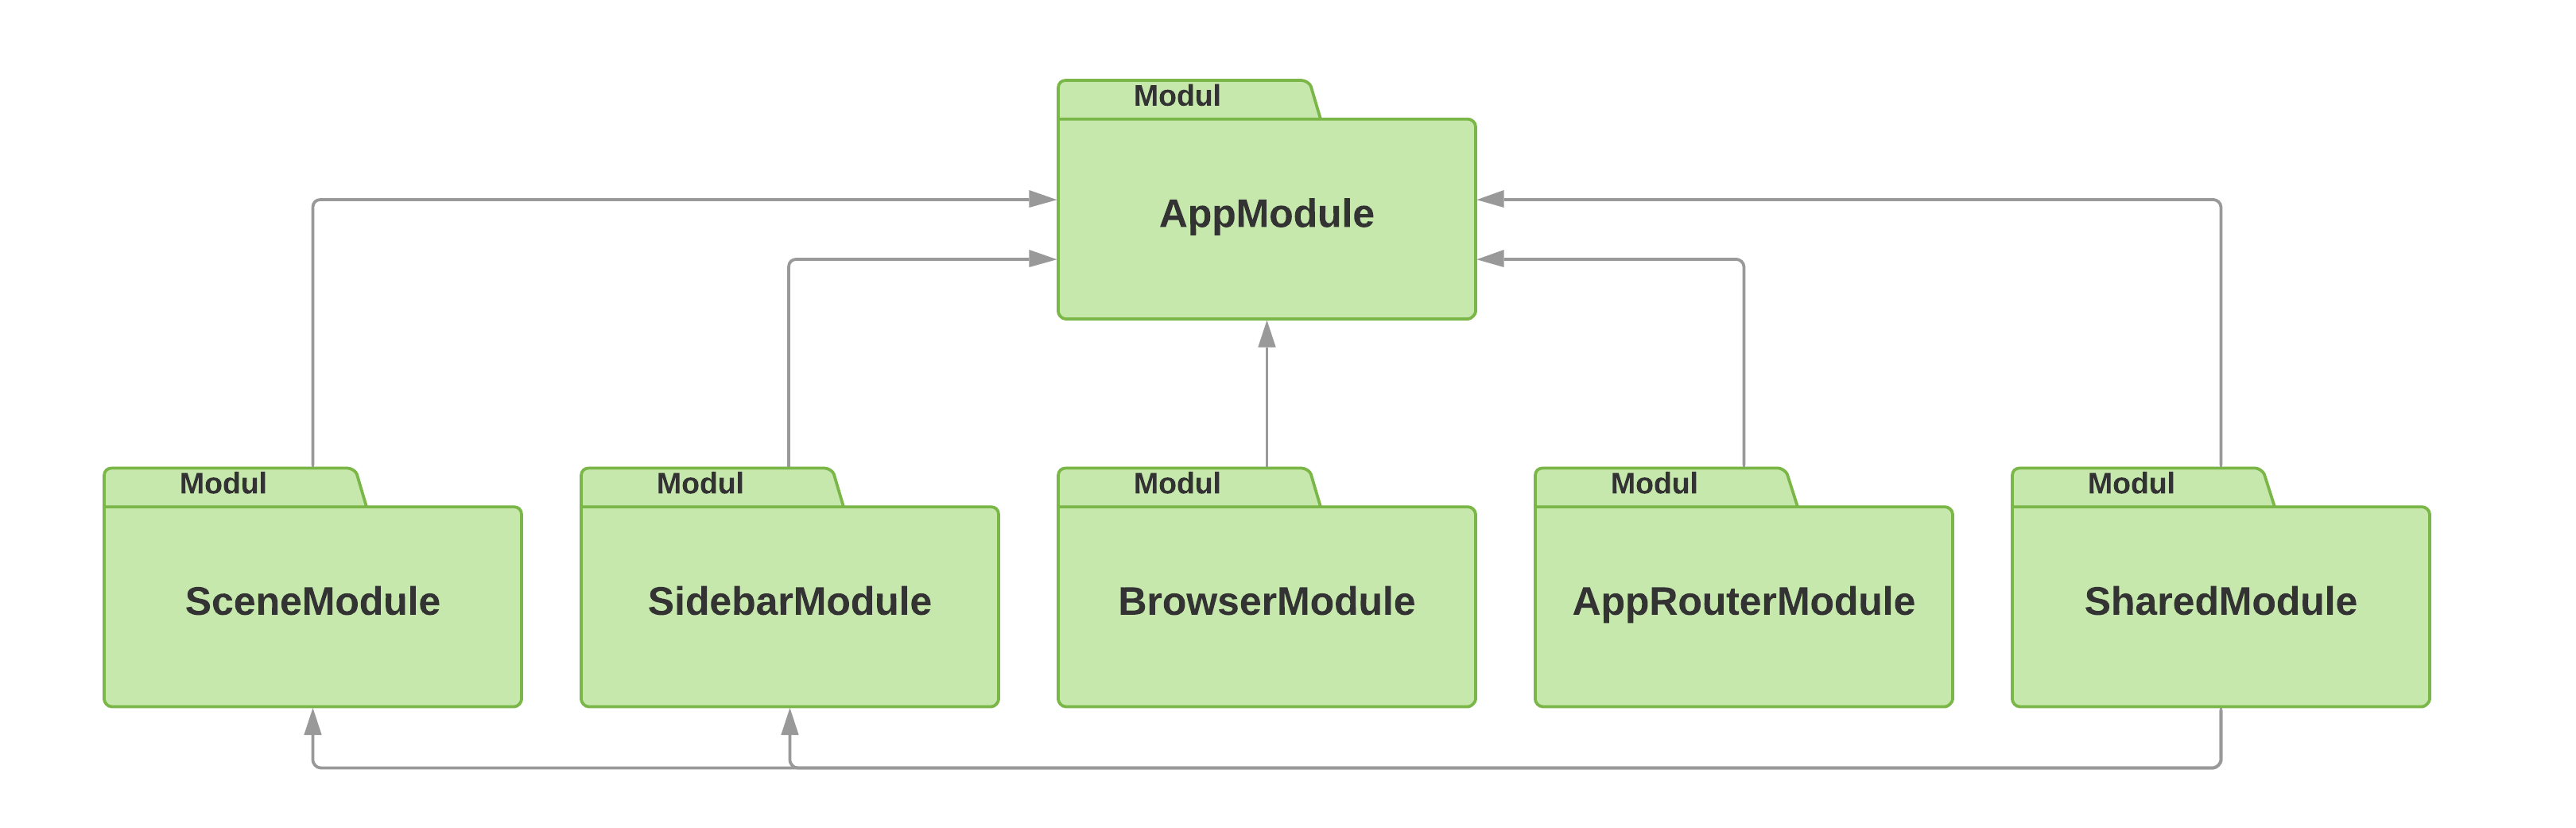
\epsfig{file = umsetzung/images/module.png, width=13.0cm}}
	\caption[Übersicht der Module]{\textit{Module der Angular-Anwendung}}
	\label{fig:module}
\end{figure}
Die einzelnen Bausteine der Angular-Anwendung werden im Rahmen dieses Bachlorprojektes immer über die Angular CLI generiert, da das am einfachsten funktioniert und zeitsparend ist. Ein Modul kann mit folgendem Command Line Befehl generiert werden:
%
\begin{lstlisting}
ng g m shared
\end{lstlisting}
%
Als Beispiel wurde hier das Module \textit{shared} angelegt. Hierin werden später alle globalen Bausteine der Angular-Anwendung erstellt. Es wurden außerdem die Appkürzungen \texttt{m} für \texttt{module} und \texttt{g} für \texttt{generate} verwendet. Ob ausgeschrieben oder abgekürzt, das hat keine Auswirkungen, sondern spart lediglich Zeit. Es gibt noch ein paar Zusatzoptionen, die als Parameter angegben werden können. Diese sind in der offizielen Dokumentation von Angular aufgeführt. Diese ermöglichen verschiedene Funktionen wie \texttt{export}-Funktion oder verhindern das generieren von Testdateien. Der 3D Konfigurator hat noch zwei weitere wichtige Module. Zum einen ist das \textit{SceneModule} für die 3D Darstellung zuständig und das Rendern des Designs. Das \textit{SidebarModule} ist sozusagen das Konfigurationsmenu inklusive einer Übersicht in tabellarischer Form. Die hauseigenen Module von Angular wie das \textit{BrowserModule} wurden von der Angular CLI automatisch importiert. Hier ist also kein weiterer Schritt notwendig, die Anwendung sollte lauffährig sein. Noch hat die Applikation allerdings noch keine richtige Funktionalität.
%
\section{Komponenten des Konfigurators}
\label{sec:umsetzung}
%
Sowohl das \textit{SidebarModule} als auch das \textit{SceneModulue} des Konfigurators haben sozusagen eine \glqq Hauptkomponente\grqq. Diese werden dann später in der \textit{AppComponent} eingebunden. Die Basis-Komponente der Anwendung ist also sehr einfach und übersichtlich. Dann gibt es noch einige weitere Kindskomponenten sowie geteilte Komponenten (aus dem \textit{sharedModule}). In diesem Kapitel werden wir uns zunächst auf die Komponenten beschränken. Alle weiteren Bausteine wie Services werden wir später noch genauer betrachten.\\
Die \textit{SceneComponent} ist dafür da die komplette 3D-Szene zu erzeugen und eben das Becher-Model mit seinem Design darstellen soll. Wie alle Kompoentente wurde diese mittels Angular CLI in PhpStorm angelegt, wie in Abbildung \ref{fig:phpstorm} zu sehen. 
%
\begin{figure}[h]
	\centering
	\subfigure[Auswahl generierbarer Angular-Bausteine]{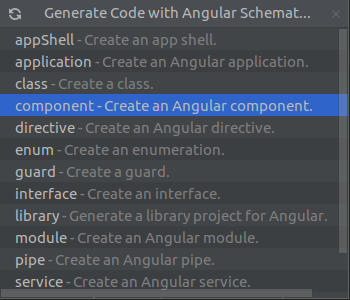
\includegraphics[width=5cm\textwidth]{umsetzung/images/auswahlcli.png}}
	\subfigure[Gernerieren einer Komponente mit Parametern]{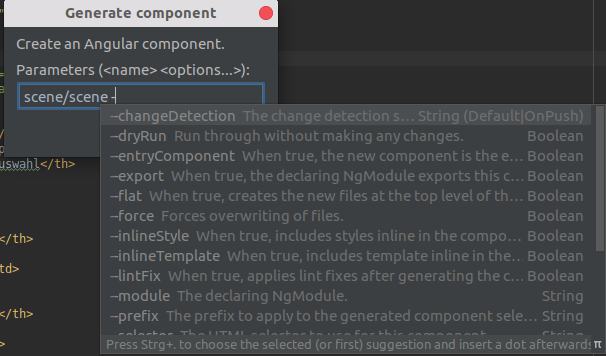
\includegraphics[width=7cm\textwidth]{umsetzung/images/optionscli.png}}\\	\subfigure[Generierte Dateien durch die CLI]{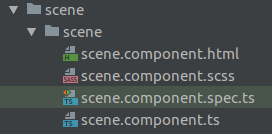
\includegraphics[width=5cm\textwidth]{umsetzung/images/generatedfiles.png}}
	\caption{\textit{Erstellung einer Angular-Komponente mit PhpStorm}}
	\label{fig:phpstorm}
\end{figure}
%
In PhpStorm kann man über \lstinline{File > New > Angular Schematics} innerhalb des Editors die Angular CLI verwenden. Wie im ersten Bild zu sehen, lassen sich so alle Bausteine von Angular anlegen. In diesem Fall wird eine Komponente angelegt. Nach der Auswahl wird man nun aufgefordert den Komponenten-Namen sowie optionale Parameter mit anzugeben. Das praktische ist, das PhpStorm alle verfügbaren Parameter vorschlägt und man nicht etwa in der Documentation nachschauen müsste, welchen Parameter man braucht und vermeidet Tippfehler. Nach bestätigen der Eingabe werden nun wie in Bild c) zu sehen alle erforderlichen Dateien der Komponente generiert. Zusätzlich werden im Hintergrund eventuelle Import-Anweisungen sowie Export- Anweisungen und so weiter automatisch ergänzt. In unserem Fall wurden auch die Testdatei erzeugt, welche wir uns im nächsten Kapitel genauer anschauen wollen. Die anderen drei Dateien sind wie wir wissen für Logik, Styles und Templating zuständig. Analog zu dem Erstellen der Komponente in PhpStorm funktioniert das ganze auch in einem Terminal:
%
\begin{lstlisting}
ng g c scene/scene -m=scene
\end{lstlisting}
%
Sobald die Komponente angelegt ist, hat sich eigentliche keine Funktionalität. Das wird erst später mit der Logik und den Services implementiert. Für den Anfang reicht es, hier schonmal das \texttt{canvas}-Element anzulegen und ein paar Styles in der \texttt{scss}-Datei der Komponente anzulegen. Wer sich mit \texttt{scss} bzw. \texttt{sass} auskennt, kann hier die Schreibweise nutzen. Man kann aber auch normales \texttt{css} schreiben. Damit ist die \textit{SceneComponent} im Grunde schon fertig.
\paragraph{Kindskomponente}
Genauso wie die \textit{SceneComponent} wurde auch die \textit{SidebarComponent} angelegt. Sie stellt die komplette Sidebar im rechten Bereich dar, also das Konfigurationsmenü und die Übersicht. Diese Komponente ist etwas komplexer und hat noch ein paar Kindskomponenten. Die Sidebar ist mit der Bootstrap-Komponente \textit{Tabs}\footnote{https://getbootstrap.com/docs/4.0/components/navs/\#tabs} umgesetzt. Wir haben also im Menu zwei Tabs, Konfigurator und Übersicht. Diese Tabs sind als eigene Komponente in \textit{SharedModule} implementiert und können in unserer SidebarCompontent also Kindskomponente verwendet werden. Es ist sozusagen ein eigener Typ für \textit{Tabs} definiert. Die Umsetzung der Tab-Komponente wird nun genauer beleuchtet.\\

Die Tabs von Bootstrap sind in einem \texttt{<ul>}-Element implementiert, welcher sozusagen den Container darstellt. Die einzelnen Tabs sind dann \texttt{<li>}-Elemente und werden durch die Liste gebündelt. Am Ende entsteht folgendes Template für die Tabs-Komponente:
%
\begin{lstlisting}
<ul class="nav nav-tabs nav-fill">
	<li class="nav-item" *ngFor="let tab of tabs" (click)="selectTab(tab)">
		<a [class.active]="tab.active" class="nav-link nav-title" href="#">{{tab.title}}</a>
	</li>
</ul>
<ng-content></ng-content>
\end{lstlisting}
%
Die \texttt{<ul>}-Liste hat ein paar vordefinierte Bootstrap-Klassen, auf die hier nicht weiter eingegangen wird. Sobald ein Tab aktiv ist, soll der dazugehörige Inhalt angezeigt werden. Wie im Quellcode zu sehen gibt es nur ein \texttt{<li>}-Tag, was nicht heißt, das es nur einen Tab gibt. Die Komponente sollte eine beliebige Anzahl an Tabs haben können. Das ist in diesem Fall dynamisch realisiert. Mit der Direktive \texttt{*ngFor} wird geprüft, wie viele Tabs im Template erstellt wurden und gibt diese dann mithilfe der for-Schleife aus. Damit wird allerdings noch nicht der Inhalt des aktiven Tab angezeigt. Dazu wird noch die \texttt{selectTab()}-Funktion benötigt. Bei \texttt{onClick} wird diese ausgeführt und teilt der Komponente mit, welcher Tab aktiv ist. Anschließend wird der Content durch \texttt{<ng-content>} ausgegeben. Um nun die Tabs als Komponente zu verwenden brauchen wird noch ein Tab-Komponente. Die Tabs-Komponente definiert, wie die Navigation insgesamt aufgebaut ist und die Tab-Komponente beschreibt, wie die einzelnen Tabs aufgebaut sind. Im Grunde werden hier nur die Inhalte des Tabs in einem div ausgegben. Wie oben im Quellcode zu sehen greifen wir auf die Variable \texttt{tab.active} und \texttt{tab.title} zu. Diese sind in Tab definiert. In unserer Sidebar würde die Tabs folgendermaßen verwendet:
%
\begin{lstlisting}
<gc-tabs>
	<gc-tab [tabTitle]="'Konfigurator'">
		Content 1
	</gc-tab>
	<gc-tab [tabTitle]="'Overview'">
		Content 2
	</gc-tab>
</gc-tabs>
\end{lstlisting}
%
Es könnten nun noch beliebig viele \texttt{<gc-tab>}-Elemente hinzugefügt werden und sie würden auch als Tab angezeigt werden. Nun ist bei jedem Tab ein \textit{title} angegben, der als Titel im Tab angezeigt werden soll. Dieser lässt sich in der Tab-Klasse über \texttt{@input} in der Variable \texttt{title} speichern und kann so an der richtigen Stelle ausgegben werden. Damit ist Tabs-Komponente funktionsfähig. Die Tabs werden dargestellt und bei onClick wird der entsprechende Tab-Inhalt angezeigt. In Abbildung \ref{fig:sidebar} ist das Endergebnis zu sehen.\\
\begin{figure}[h]
	\centering
	{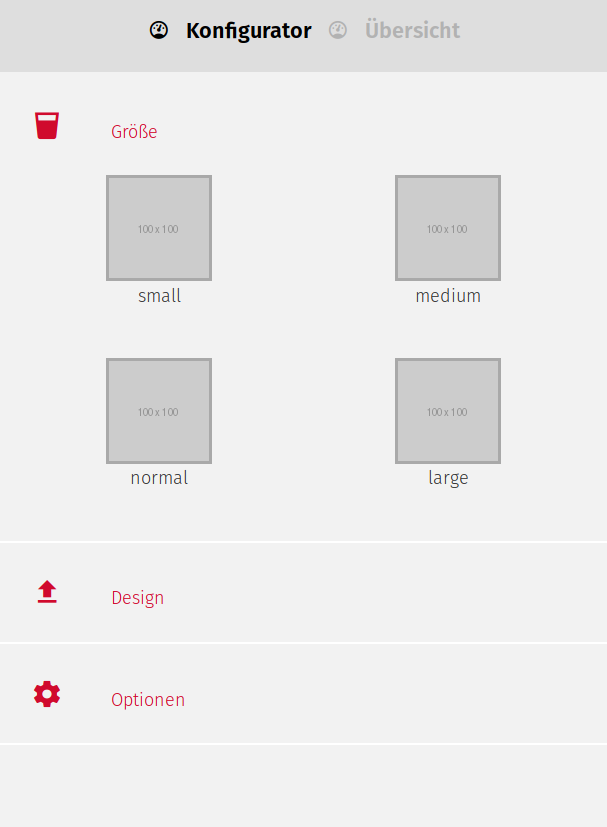
\epsfig{file = methodik/images/sidebar.png, width=8.0cm}}
	\caption[Sidebar des Konfigurators]{\textit{Sidebar der Angular-Anwendung}}
	\label{fig:sidebar}
\end{figure}


Zusätzlch hat die SidebarComponent auch noch eigene nicht geteilte Kindskompontenten. Das Konfigurationsmenü besteht aus Größe, Design-Upload und Optionen. Diese drei sind ebenfalls als Menü umgesetzt. Es handelt sich hier wieder um eine Bootstrap Komponente, das Accordion, welches ein aufklappbares Menü ist (\textit{Collapse})\footnote{https://getbootstrap.com/docs/4.0/components/collapse}. Die einzelnen Punkte sind hier auch wieder eigenständige Komponenten die als Kindskomponenten in der \textit{SidebarComponent} verwendet werden. Allerdings sind diese Komponenten weniger komplex. Hier sind alle Menüpunkte unterschiedlich aufgebaut, weshalb es 3 verschiedene Komponenten gibt. Das Accordion wird wie in der Dokumentation von Bootstrap verwendet. Wie das ganze am Ende aussieht kann man auch in Abbildung \ref{fig:sidebar} sehen. Die Komponenten \texttt{<gc-size>}, \texttt{<gc-upload>}, und \texttt{<gc-options>} sind dann sozusagen der Content. Die \textit{SizeComponent} und \textit{OptionsComponent} sind einfache \texttt{html}-Snippets. Die \textit{UploadComponent} ist wegen dem Upload-Vorgang des Designs etwas komplexer und wird später noch genauer beschrieben.
%
\section{3D Szene mit Model}
\label{sec:umsetzung}
%
\paragraph{Szene erstellen}Die \textit{SceneComponent} wurde schon angelegt. Nun muss noch die Funktionalität programmiert werden. In unserem Template ist alles was wir brauchen ein \texttt{<canvas>}-Element, \textbf{(ElementRef als Service erwähnen) }in dem dann später die ganze 3D Szene dargestellt wird. Zum Erstellen der 3D Szene und dem Laden der 3D-Models wird ein Service verwendet. Dieser Angular Baustein kann auch über die CLI angelegt werden. Der Service hat nun eine \texttt{createScene()} Funktion, die eine Scene mit Belichtung und Kamera erzeugt. Ihr wird als Parameter das \texttt{<canvas>}-Element übergeben. Für den Konfigurator wurden verschiedene Belichtungen verwendet, die ein optimales Licht erzeugen. Dabei handelt es sich um ein \textit{AmbientLight}, \textit{KeyLight}, \textit{FillLight} und \textit{BackLight}. Die Kamera hat verschiedene Werte zugewiesen bekommen, damit sie in der richtigen Perspektive den Becher später darstellt.
%
\paragraph{Model laden} Nun fehlt es noch an Leben in der Szene. Als 3D Model werden testweise Becher verwendet, die in etwa den späteren Mehrwegbechern entsprechen. Die 3D Models sind einfach \texttt{.obj}-Dateien, die aus 3D Programmen exportiert werden können. Mithilfe des \textit{OBJ-Loaders} kann man nun die Datei in die Szene laden. Jedoch stößt man da schnell auf das Problem, das die Loader nicht standardmäßig implementiert sind. Abhilfe schafft hier das \textit{npm}-Module \textit{full-three}\footnote{https://www.npmjs.com/package/three-full}. Es beeinhaltet die komplette Three.js Bibliothek mit allen Beispielen und Loadern. Nachdem also die Szene mit Kamera und Belichtung steht, wird die \texttt{.obj}-Datei geladen.
%
\begin{lstlisting}
const loader = new THREE.OBJLoader();
loader.load('assets/model/test.obj', this.onModelLoadingCompleted);
\end{lstlisting}
%
In der Funktion \texttt{onModelLoadingCompleted} wird dann der Renderer ausgeführt, die das Model zur Szene hinzufügt und anschließend alles rendert. Jetzt ist die 3D Ansicht schon mal mit Leben gefüllt, der nackte Becher angezeigt wird (siehe Abbildung \ref{fig:3dmodel}).
\begin{figure}[h]
	\centering
	{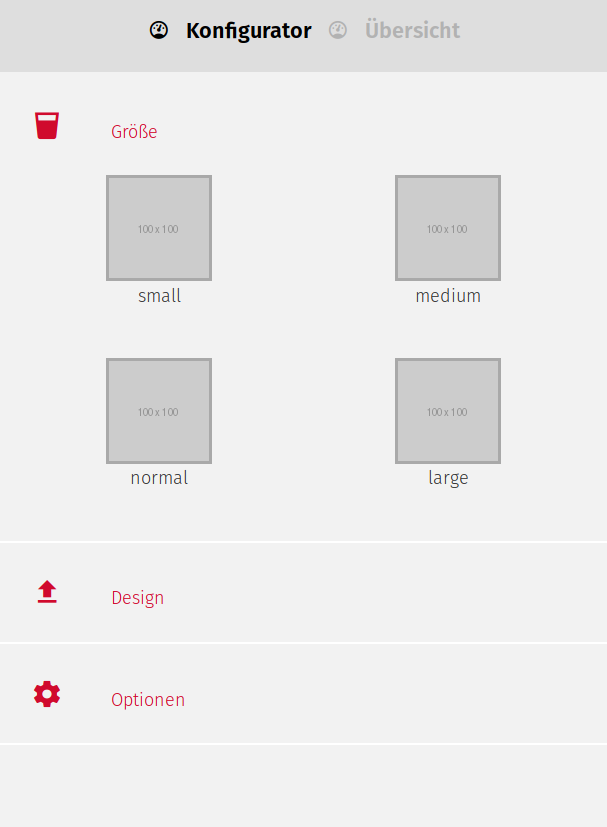
\epsfig{file = methodik/images/sidebar.png, width=8.0cm}}
	\caption[Komponentendiagramm]{\textit{Sidebar der Angular-Anwendung}}
	\label{fig:3dmodel}
\end{figure}
\paragraph{Auswahl der Größe}
Unter dem Menüpunkt \textit{\glqq Größe\grqq} soll der Benutzer eine der vier Größen wählen. Standardmäßig ist von Beginn an der 0,2 Liter Becher gewählt und ist von Angfang an sichtbar. Wie genau der DataService funktioniert, wird später noch einmal genauer beleuchtet. Zunächst werden in der \texttt{<gc-size>}-Komponente die verschiedenen Auswahlmöglichkeiten dargestellt. Mit der \texttt{onClick}-Funktion \texttt{reloadModel()} wird dem \textit{SceneService} mitgeteilt, das der Benutzer eine Bechergröße gewählt hat. 
%
\begin{lstlisting}
this.scene.remove(currentModel);

const loader = new THREE.OBJLoader();
const file = 'assets/model/' + model + '.obj';
loader.load(file, this.onModelLoadingCompleted);

this.controls.update();
this.render();
\end{lstlisting}
%
In der Funktion wird als erstes das aktuelle Model entfernt. Danach wird geprüft, welche Größe der User ausgewählt hat und dementsprechend wird das neue Model geladen. Anschließend muss die Szene neu gerendert werden. 
\paragraph{Controlling}
Der Becher soll in 3D angezeigt werden und soll rotiert werden können. In Three.js wird dafür \textit{OrbitControl} verwendet. Diese Klasse liefert verschiedene Werte mit, die verschiedene Einstellungen ermöglichen. Beispielsweise kann man die Rotationsgeschwindigkeit einstellen. Wenn man den Becher im Extremwinkel betrachtet oder zu weit hineinzoomt, kann der Becher bzw. dessen Texture unscharf aussehen oder nicht realistisch dargestellt sein. Deshalb wird über die Controls auch ein maximaler Zoom und ein maximaler Betrachtungswinkel festgesetzt.
\paragraph{Responsive} Die Ansicht sollte auf allen Displaygrößen darstellbar sein. Dafür sorgt der \texttt{@HostListener}. Dieser macht nichts anderes als die Fenstergröße zu überprüfen und das \texttt{<canvas>}-Element anschließend an den Container anzupassen. Falls sich die Fenstergröße ändert, wird der Szene über die Funktion \texttt{getAspectRatio()} die aktuelle Größe übermittelt. Dann wird die Szene aktualisiert und neu gerendert. Damit ist verhindert, das zum Beispiel auf kleineren Geräten der Becher abgeschnitten dargestellt wird oder ähnliches.
%
\section{Design Rendering}
\label{sec:umsetzung}
%
Jetzt geht es um das Hauptproblem der Arbeit: Auf dem Becher muss das Design des Kunden gerendert werden. Zunächst wird zum Testen ein Design erstellt, so wie es der Kunde hochladen würde. Nach verschiedenen Test, das Design direkt auf den Becher als Textur zu rendern wurde eine besser Lösung gefunden. 
\paragraph{3D Zylinder}
Die Bibliothek Three.js kann Geometrien erzeugen. Das heißt, man muss kein 3D Model aus einer Datei laden, sondern kann im Code eine geometrische Form erzeugen. Genau das wird für das Design des Bechers genutzt. Der Becher hat die Form eines Zylinders. Innerhalb der \texttt{onModelLoadingCompleted}-Funktion wird nun eine \textit{CylinderBufferGeometry}\footnote{https://threejs.org/docs/\#api/en/geometries/CylinderBufferGeometry} erstellt. Im Grunde umhüllt das Design den Becher wie ein Aufkleber.
%
\begin{lstlisting}
const geometry = new THREE.CylinderBufferGeometry(<radiusOben>, <radiusUnten, <height>, <radialSegmente>, <heightSegmente>, <offenesEnde>, <lenght>);
\end{lstlisting}
%
Durch die Parameter ist es möglich, den Zylinder genau an die Maße des Bechers anzupassen. Er liegt ganz eng auf dem Becher, eben wie ein Aufkleber. Mit dem Parameter \texttt{<offenesEnde>} wird festgelegt, das der Cylinder hohl ist und \texttt{<lenght>} stellt sicher, das der Zylinder 360 Grad im den Becher dargestellt wird.\footnote{Um das zu erreichen setzt man einfach den Wert auf \textit{2*Pi }}. Die anderen Parameter beschreiben den Radius und die Höhe des Zylinders. Im \textit{ThreeService} sind die Parameter der \textit{CylinderBufferGeometry} in Variablen für jeden der vier Becher definiert. Bevor die Geometrie erstellt wird, muss nur das aktuelle Model geprüft werden .Dann müssen die passenden Zylinder-Parameter für die aktuelle Bechergröße geladen werden. Somit umhüllt der Zylinder immer den ganzen Becher, egal welche Bechergröße gewählt ist.\\
Jetzt kann das Design des Kunden als Texture auf den Zylinder gepackt werden. Das praktische ist, das sich das Design an die Maße des Zylinders anpasst. Wenn das Design in der richtigen Auflösung hochgeladen wurde, sieht es somit realistisch aus\footnote{Im Upload-Vorgang wird der Benutzer bei falscher Auflösung des Designs darauf hingewiesen (siehe Kapitel 5.9).}. Aufgrund der kubischen Form des Zylinders wird das Design minimal gestaucht, genau wie beim Druck.
\begin{figure}[h]
	\centering
	{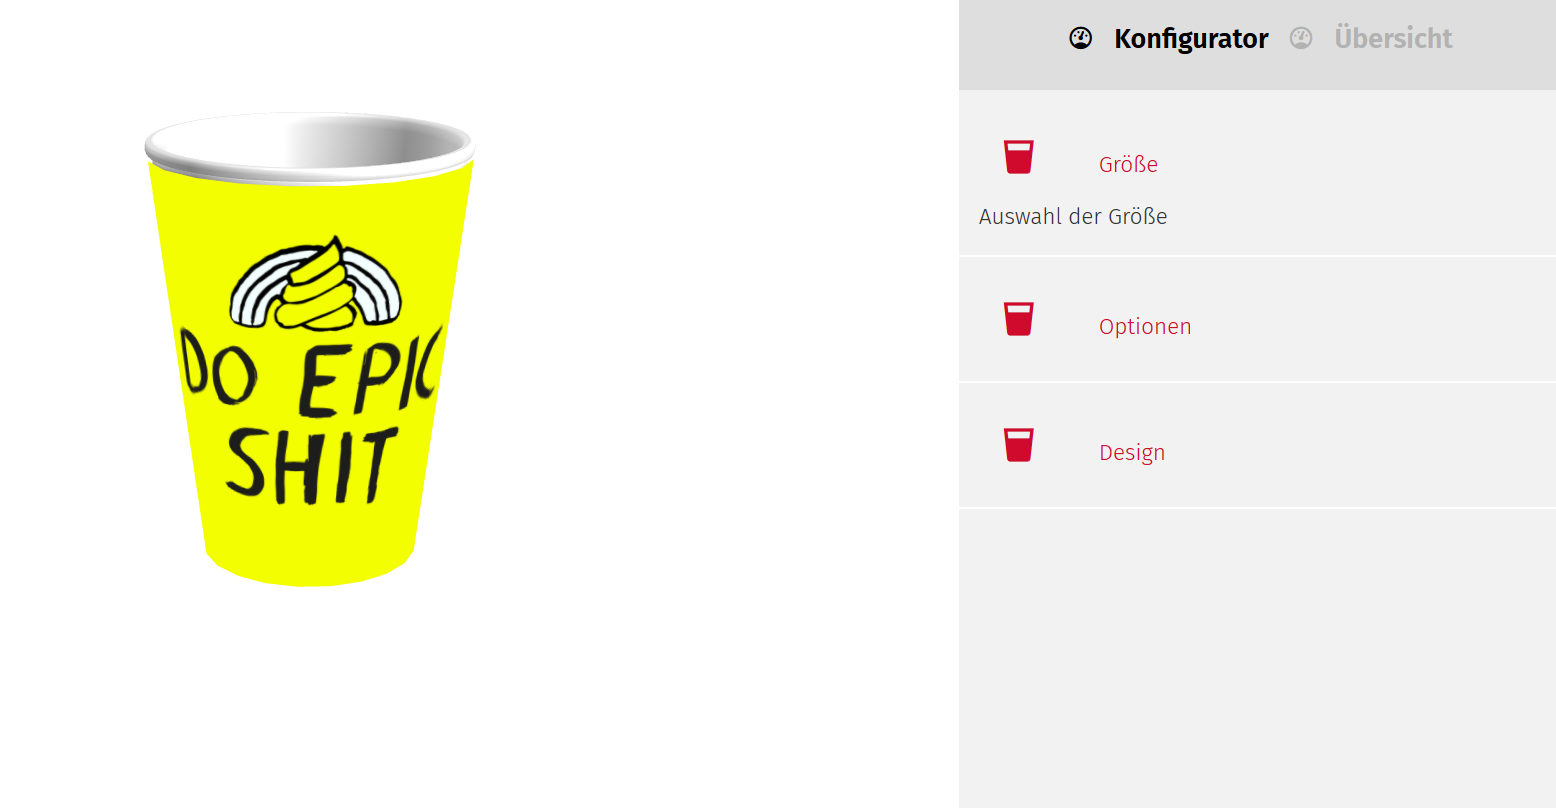
\epsfig{file = umsetzung/images/bechermitdesign.PNG, width=11.0cm}}
	\caption[Konfigurator mit designtem Becher]{\textit{Darstellung des Designs auf dem Becher mit Zylinder-Geometrie}}
	\label{fig:bechermitdesign}
\end{figure}
Da der Upload des Designs noch bis hierhin noch nicht implementiert ist, wird mit einem statischen Design gearbeitet. In Kapitel 5.9 wird sich diese Arbeit mit dem Upload-Vorgang beschäftigen. Solange allerdings kein Design als Texture hochgeladen wurde, wird der erstellte Zylinder in der Scene ausgeblendet. Es würde keinen Sinn machen einen blanken Zylinder um den Becher anzuzeigen. Die 3D Darstellung des Bechers mit Design funktioniert aber grundsätzlich schon, wie man in Abbildung \ref{fig:bechermitdesign} sehen kann.
%
\section{Mobile Umsetzung}
\label{sec:umsetzung}
%
Auf Tablets (in der Portraitansicht) ist es praktisch das Menü unterhalb der 3D Ansicht darzustellen. Das lässt sich ganz einfach mit den Column-Klassen von Bootstrap realisieren. Interessanter wird die Darstellung auf Smartphones.\\
Das Off-Canvas Menu ist vom Design nicht anders als die Desktop-Variante. Es wird lediglich verschoben. Das bedeutet, wenn ein Benutzer auf dem Smartphone den Konfigurator öffnet, sieht er zunächst nur den 3D Becher. Er kann dann das Off-Canvas-Menu über ein Hamburger-Menu-Button öffnen. Das ganze ist mit einer JavaScript Funktion realisiert, die einfach das Menü aus dem sichtbaren Bereich verschiebt und sie erst dann sichtbar werden lässt, wenn der Hamburger-Menu-Button gedrückt wird. Über \texttt{css} werden die SceneComponent sowie die SidebarComponent noch so angepasst, dass sie immer 100\% des Displays einnehmen. Außerdem werden die Schriftgrößen etwas größer gemacht.
Der Hamburger-Button ist ausschließlich auf Smartphones sichtbar. Wenn dieser geklickt wird, greift die Funktion \texttt{showsidebar()} bzw. \texttt{hideSidebar()}.
%
\begin{lstlisting}
document.getElementById("mySidenav").style.width = 100%;
\end{lstlisting}
%
Soll die Sidbar angezeigt werden, wird die Höhe auf \texttt{100\%} gesetzt. Soll sich geschlossen werden, wird die Breite auf \texttt{0} gesetzt. Damit ist eine sehr simple Lösung einer mobilen Sidebar implementiert.

Die 3D Szene ist, wie schon zuvor erwähnt, auch responsive. Die OrbitControls von Three.js liefern auch eine Kompatiblität für Touch-Eingaben mit. So kann auf mobilen Geräten der Becher via Touch rotiert werden.
%
\section{Daten-Service}
\label{sec:umsetzung}
%
Der DataService hat eine Aufgabe: Alle Daten des konfigurierten Bechers zu speichern und sie bei Anfrage einer Komponente wieder zurückzugeben. Dabei ist es wichtig das der Service nur einmal gestartet wird und die Daten global speichert. Hierbei handelt es sich also um ein Singelton. In Angular einen Service zu implementieren, ist recht unkompliziert. Analog zum \textit{SceneService} wird dieser auch über Angular CLI anzulegen. Anders als der \textit{SceneService}, welcher ausschließlich von der \textit{SceneComponent} verwendet wird, soll dieser global zugänglich sein. Dabei speichert er folgende Daten:
\begin{description}
	\item[selectedImage] Speichert die \texttt{png}-Datei, welche der User hochgelden hat
	\item[state] Hat den Wert \textit{true} wenn ein Bild ausgewählt wurde
	\item[designName] Speichert den Namen der Bilddatei
	\item[designSize] Speichert die Größe der Bilddatei
	\item[count] Speichert die Anzahl der Becher, die der Benutzer später drucken lassen möchte 
	\item[size] Speichert die vom Benutzer gewählte Bechergröße
	\item[stroke] Speichert, ob der Eichstrich mitgedruckt werden soll (Optionale Auswahl)
	\item[price] Zeigt den aktuellen Staffelpreis abhängig der gewählten Anzahl.
	\item[model] Speichert den Pfad zur \texttt{.obj}-Datei, welche gerendert werden soll
\end{description}
%
Die Eigenschaften \textit{designName}, \textit{count}, \textit{size}, \textit{stroke} und \textit{price} werden in der Tabelle \textit{OverviewComponent} als Bindung angezeigt. Somit ist immer die aktuelle Auswahl des Benutzers in der Tabelle. \\
Der \textit{DataService} ist somit ein Speicherort aller Informationen über den ausgewählten Becher und das verwendete Design. Es ist durchaus denkbar den Service später zu erweitern. Man könnte die Informationen auf einem Server sichern, sodass der User zu späteren Zeiten auf seine Konfiguration zurückgreifen kann. Angular bitet dafür eine einfache Realisierung über das \textit{HttpClientModule}.

Auch der \textit{SceneService} nutzt den \textit{DataService}. Zunächst bekommt der \textit{SceneService}, wie schon erwähnt, die Information, welche Größe gewählt wurde. Je nach dem welchen Wert \textit{size} dann hat, ändert sich das 3D-Model. Ähnlich verhält es sich mit dem Design, was als Textur auf dem Becher angezeigt werden soll. Im nächsten Abschnitt wird genauer beschrieben, wie ein Design hochgeladen werden kann, und welche Rolle der \textit{DataService} dort spielt.
%
\section{Upload-Vorgang}
\label{sec:umsetzung}
%
Angenommen ein Benutzer hat sich für eine Größe entschieden und möchte nun sein Design auswählen. In der Sidebar kann über einen Button die \textit{UploadComponent} geöffnet werden. Der User wird hier auch noch einmal darauf hingewiesen, die Druckvorgaben zu beachten.
\paragraph{Route zum Upload}
An dieser Stelle der Anwendung wird das \textit{Routing} verwendet. Normalerweise befinden wir uns in dem Konfigurator unter dem root-Pfad. Beim Upload ändert sich der Pfad zu \texttt{localhost/upload}. Unter dieser Route ist definiert, das die \textit{UploadComponent} angezeigt werden soll und nicht die \textit{SidebarComponent}. Hier kann der Benutzer jetzt sein Design auswählen (siehe Abbildung).
%
\begin{figure}[h]
	\centering
	{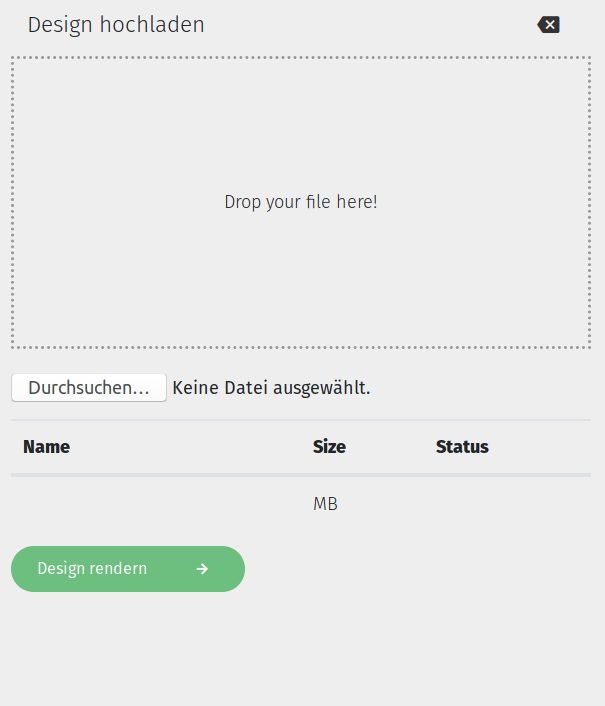
\epsfig{file = umsetzung/images/uploadcomponent.png, width=8.0cm}}
	\caption[UploadComponent des Konfigurators]{\textit{Upload-Komponente der Angular-Anwendung zum auswählen des Designs}}
	\label{fig:sidebar}
\end{figure}
%
Eigentlich ist der Begriff \glqq Upload \grqq nicht ganz zutreffend, da das Design nicht wirklich auf einen Server hochgeladen wird, sondern nur in dem \textit{DataService} gespeichert wird. Trotzdem ist klar, was die Funktion dieser Komponente ist. Der Benutzer hat zwei Möglichkeiten sein Design auszuwählen.
%
\paragraph{Drag \& Drop oder Select}
Eine bekannte Methode um Dateien hochzuladen ist die Drag \& Drop Methode. Man muss einfach die Datei in den dafür vorgesehenen Bereich ziehen und die Datei wird erkannt. Die zweite Möglichkeit ist es ganz klassisch über ein Input-Feld eine Datei aus dem Verzeichnis auszuwählen. Egal, für welche Methode der Benutzer sich entscheidet, passiert im Grunde das selbe. Ein Unterschied besteht darin, das verschiedene Eregnisse gebunden werden. Bei der klassischen Input-Feld Variante wird über das Event \textit{Change} überprüft, ob eine Datei ausgewählt wurde. Bei der Drag \& Drop Variante wird das Event \textit{drop} verwendet. Außerdem wird zusätzlich \texttt{dragover} und \texttt{dragleave} ausgeführt, wenn eine Datei in die Dropzone gezogen wird oder hinausgezogen wird. Für eine bessere Usability verändern sie die Farbe des Rahmens. Somit bekommt der User ein Feedback, wenn er seine Datei an die richtige Stelle gezogen hat.


In der \textit{UploadComponent} sind beide Upload-Vorgänge mit der Direktiven umgesetzt. In Diesen sind Dekoratoren implementiert, welche die eben erwähnten  Ereignisse über \texttt{@Hostlistener} binden. Für den Upload-Vorgang in diesem Konfigurator wird ein benutzerdefiniertes Ereignis benötigt. Um das zu erstellen verwendet man das \texttt{EventEmiter}-Objekt.
%
\begin{lstlisting}
private filesChangeEmiter: EventEmitter<File> = new EventEmitter();
\end{lstlisting}
%
Zusätzlich muss der Typ der Objekte explizit festgelegt werden. In diesem Fall wird ein \texttt{File}(einfache Datei) emittiert, jedes Mal, wenn der Benutzer eine Datei ausgewählt hat. Da der User nur ein Bild hochladen darf, ist dies nicht als Array implementiert. Nun können wir den \textit{EventEmiter} in \textit{@HostListener} verwenden. Es muss aber noch das Ereignis mit der übergeordneten HTML-Komponente gebunden werden. Dazu benötigt man den \textit{@Output} Dekorator für den \textit{EventEmiter}. Auf diese Weise ist es möglich zu überprüfen, ob sich die ausgewählte Datei geändert hat.
%
\begin{lstlisting}
<div gcDragDrop (filesChangeEmiter)="onFilesChange($event)">
\end{lstlisting}
%
Wie man im Beispiel sieht, wird jedes Mal, wenn eine Datei in die Drop-Zone geschoben wird, die Funktion \texttt{onFilesChange(\$event)} ausgeführt. Der Parameter \texttt{\$event} ist immer ausgewählte Datei. Die Methode kann jetzt mit diesem File arbeiten.\\

In der \textit{UploadCompontent} und auch an anderen Stellen der Anwendung soll der Dateiname und die Größe der Datei ausgegeben werden. Es ist nun möglich aus der übergebenen Datei beides auszulesen und in dem \textit{DataService} zu speichern. Nun muss noch die \texttt{reloadTexture()}-Funktion ausgeführt werden und die Datei übergeben werden. In Three.js werden Texturen mit dem TextureLoader geladen bzw. gemappt. Anschließend kann man sie zur Szene hinzufügen. Allerdings kann der Loader nur URLs oder Base64-Objekte entgegen nehmen. Auf den Pfad des Bildes können wir aus Sicherheitsgründen nicht zugreifen. Deshalb muss das File-Objekt in ein Base64-Objekt konvertiert werden, bevor man die Textur laden kann. Das konvertierte Objekt wird dann in \texttt{selectedImage} im \textit{DataService} gespeichert.
%
\begin{lstlisting}
this.getBase64(file).then(
	data => this.DataServ.selectedImage = data
);
\end{lstlisting}
%
Ist nun eine gültige \texttt{.png}-Datei ausgewählt worden, wird wie in Abbildung zu sehen Name und Dateigröße angezeigt. Jetzt ist auch der \textit{Design rendern}Button aktiv und das Design kann mit der \textit{reloadTexture}-Funktion gerendert werden.

\paragraph{reloadTexture}
Im Grunde ist diese Funktion nahezu identisch zu \texttt{reloadModel()}-Funktion. Ein Teil der Funktion ist schon bekannt. Wir haben schon gesehen wie diese Funktion den Zylinder für das Design um den Becher erstellt. Als Erstes löscht die Funktion eine Texture, die eventuell schon zuvor gerendert wurde. Nun bekommt die Funktion das Design des Users als Parameter übergeben und kann es als Texture gemappt werden.
%
\begin{lstlisting}[caption={TextureLoader Umsetzung},label=lst:texture]
const loader = new THREE.TextureLoader();
const material = new THREE.MeshBasicMaterial();
material.map = loader.load(image);
\end{lstlisting}
%
Um das ganze abzuschließend wird nun noch die Textur mit der Geometrie zusammengeführt und schließlich zu Szene hinzugefügt. Nachdem dann die Szene neu gerendert wurde, sollte das Design des Benutzers richtig auf dem Becher angezeigt werden.\\

Damit ist die Realisierung abgeschlossen. Die Funktionen wurden weitesgehend alle implementiert und müssen jetzt noch geprüft werden.
		
		%---- Kapitel Testphase ----
		%
%%%%%%%%%%%%%%%%%%%%%%%%%%%%%%%%%%%%%%%%%%%%%%%%%%%%%%%%%%
%
%  T E S T P H A S E   &   E R G E B N I S S E
%
%%%%%%%%%%%%%%%%%%%%%%%%%%%%%%%%%%%%%%%%%%%%%%%%%%%%%%%%%%
\chapter{Testphase \& Ergebnisse}
\label{cha:testphase}
%
Unter funktionalen Anforderungen versteht man konkrekte Funktionalitäten, welche die Anwendung leisten soll. Die Anwendung lässt sich in mehrere Module aufteilen, die dem User zu Verfügung stehen. Im Folgenden werden die funktionalen Anforderungen erläutert.
		
		%---- Kapitel Zusammenfassung ----
		%
%%%%%%%%%%%%%%%%%%%%%%%%%%%%%%%%%%%%%%%%%%%%%%%%%%%%%%%%%%
%
%  Z U S A M M E N F A S S U N G
%
%%%%%%%%%%%%%%%%%%%%%%%%%%%%%%%%%%%%%%%%%%%%%%%%%%%%%%%%%%
\chapter{Zusammenfassung}
\label{cha:fazit}
%
Unter funktionalen Anforderungen versteht man konkrekte Funktionalitäten, welche die Anwendung leisten soll. Die Anwendung lässt sich in mehrere Module aufteilen, die dem User zu Verfügung stehen. Im Folgenden werden die funktionalen Anforderungen erläutert.

	%---- Beginn Anhang ----
	\appendix	% resets numbering to alphabetic style
	%
%
\chapter{Lorem Ipsum}
%
%
Lorem ipsum dolor sit amet, consectetur adipisici elit, sed eiusmod tempor incidunt ut labore et dolore magna aliqua. Ut enim ad minim veniam, quis nostrud exercitation ullamco laboris nisi ut aliquid ex ea commodi consequat. Quis aute iure reprehenderit in voluptate velit esse cillum dolore eu fugiat nulla pariatur. Excepteur sint obcaecat cupiditat non proident, sunt in culpa qui officia deserunt mollit anim id est laborum.
\\
Duis autem vel eum iriure dolor in hendrerit in vulputate velit esse molestie consequat, vel illum dolore eu feugiat nulla facilisis at vero eros et accumsan et iusto odio dignissim qui blandit praesent luptatum zzril delenit augue duis dolore te feugait nulla facilisi. Lorem ipsum dolor sit amet, consectetuer adipiscing elit, sed diam nonummy nibh euismod tincidunt ut laoreet dolore magna aliquam erat volutpat.
\\
Ut wisi enim ad minim veniam, quis nostrud exerci tation ullamcorper suscipit lobortis nisl ut aliquip ex ea commodo consequat. Duis autem vel eum iriure dolor in hendrerit in vulputate velit esse molestie consequat, vel illum dolore eu feugiat nulla facilisis at vero eros et accumsan et iusto odio dignissim qui blandit praesent luptatum zzril delenit augue duis dolore te feugait nulla facilisi.
\\
Nam liber tempor cum soluta nobis eleifend option congue nihil imperdiet doming id quod mazim placerat facer possim assum. Lorem ipsum dolor sit amet, consectetuer adipiscing elit, sed diam nonummy nibh euismod tincidunt ut laoreet dolore magna aliquam erat volutpat. Ut wisi enim ad minim veniam, quis nostrud exerci tation ullamcorper suscipit lobortis nisl ut aliquip ex ea commodo consequat.
\\
Duis autem vel eum iriure dolor in hendrerit in vulputate velit esse molestie consequat, vel illum dolore eu feugiat nulla facilisis.
\\
At vero eos et accusam et justo duo dolores et ea rebum. Stet clita kasd gubergren, no sea takimata sanctus est Lorem ipsum dolor sit amet. Lorem ipsum dolor sit amet, consetetur sadipscing elitr, sed diam nonumy eirmod tempor invidunt ut labore et dolore magna aliquyam erat, sed diam voluptua. At vero eos et accusam et justo duo dolores et ea rebum. Stet clita kasd gubergren, no sea takimata sanctus est Lorem ipsum dolor sit amet. Lorem ipsum dolor sit amet, consetetur sadipscing elitr, At accusam aliquyam diam diam dolore dolores duo eirmod eos erat, et nonumy sed tempor et et invidunt justo labore Stet clita ea et gubergren, kasd magna no rebum. sanctus sea sed takimata ut vero voluptua. est Lorem ipsum dolor sit amet. Lorem ipsum dolor sit amet, consetetur sadipscing elitr, sed diam nonumy eirmod tempor invidunt ut labore et dolore magna aliquyam erat.
\\
Consetetur sadipscing elitr, sed diam nonumy eirmod tempor invidunt ut labore et dolore magna aliquyam erat, sed diam voluptua. At vero eos et accusam et justo duo dolores et ea rebum. Stet clita kasd gubergren, no sea takimata sanctus est Lorem ipsum dolor sit amet. Lorem ipsum dolor sit amet, consetetur sadipscing elitr, sed diam nonumy eirmod tempor invidunt ut labore et dolore magna aliquyam erat, sed diam voluptua. At vero eos et accusam et justo duo dolores et ea rebum. Stet clita kasd gubergren, no sea takimata sanctus est Lorem ipsum dolor sit amet. Lorem ipsum dolor sit amet, consetetur sadipscing elitr, sed diam nonumy eirmod tempor invidunt ut labore et dolore magna aliquyam erat, sed diam voluptua. At vero eos et accusam et justo duo dolores et ea rebum. Stet clita kasd gubergren, no sea takimata sanctus est Lorem ipsum dolor sit amet.

	%---- Ende Anhang ----

	\cleardoublepage



	% ---- the backmatter ----
	\backmatter
	
		%---- include Glossar ----
		%
%%%%%%%%%%%%%%%%%%%%%%%%%%%%%%%%%%%%%%%%%%%%%%%%%%%
%
% G L O S S A R
%
%%%%%%%%%%%%%%%%%%%%%%%%%%%%%%%%%%%%%%%%%%%%%%%%%%%
\chapter{Glossar}
\label{cha:glossar}


\begin{tabular}{p{3cm} p{12cm}}

\textbf{CLI} & Command Line Interface\\
\\
\textbf{SEMVER} & Semantische Versionierung \\
\\
\textbf{UML} & Unified Modeling Language \\
\\
\end{tabular}


		%---- Literaturverzeichnis ----
%		\begin{footnotesize}
			\bibliography{abschlussarbeit}
			\bibliographystyle{alphadin}
%		\end{footnotesize}
		
		%---- Own publications again ----
		\cleardoublepage

		%---- Indexverzeichnis ----	
		\cleardoublepage
%		\pagestyle{index}
%		\renewcommand{\chaptermark}[1]{}
		\renewcommand{\preindexhook}{ % Die erste angegebene Seitenzahl ist gewöhnlich, aber nicht immer, die erste Referenz zum entsprechenden Eintrag.
		\vskip\onelineskip}
		\indexintoc
		\printindex
		\cleardoublepage

	
\end{document}
